\documentclass[11pt,letterpaper]{article}
\usepackage[margin=.78in,headheight=15pt,footskip=29pt]{geometry}
\usepackage[T1]{fontenc}
\usepackage{newtxtext,newtxmath,fontspec}
\setsansfont{texgyreheros-regular.otf}[BoldFont=texgyreheros-bold.otf]
\usepackage[table]{xcolor}
\usepackage{microtype,graphicx,tikz,booktabs,longtable,array,tabularx,amsmath}
\usetikzlibrary{positioning,arrows.meta,fit,backgrounds}
\usepackage{enumitem,titlesec,fancyhdr,lastpage,needspace,caption,float,xurl}
\usepackage[colorlinks=true,linkcolor=teal,urlcolor=teal]{hyperref}
\hypersetup{pdftitle={Seven-model coding benchmark - Muse attention decode},pdfauthor={} ,pdfsubject={Derived public scientific results}}
\definecolor{navy}{HTML}{183249}
\definecolor{teal}{HTML}{087F8C}
\definecolor{gold}{HTML}{D89A24}
\definecolor{purple}{HTML}{7954A1}
\definecolor{muted}{HTML}{53616D}
\definecolor{pale}{HTML}{F0F4F7}
\definecolor{grid}{HTML}{D6DEE5}
\setlength{\parindent}{0pt}
\setlength{\parskip}{5pt}
\setlength{\emergencystretch}{2em}
\setlength{\tabcolsep}{4pt}
\renewcommand{\arraystretch}{1.16}
\setlist{leftmargin=1.35em,itemsep=3pt,topsep=4pt}
\titleformat{\section}{\Large\sffamily\bfseries\color{navy}}{\thesection}{.6em}{}
\titleformat{\subsection}{\large\sffamily\bfseries\color{teal}}{\thesubsection}{.6em}{}
\titlespacing*{\section}{0pt}{16pt}{7pt}
\captionsetup{font=small,labelfont={bf,sf,color=navy},textfont={color=muted}}
\pagestyle{fancy}\fancyhf{}
\fancyhead[L]{\small\sffamily\color{muted}MUSE ATTENTION DECODE}
\fancyhead[R]{\small\sffamily\color{muted}Public scientific projection}
\fancyfoot[L]{\scriptsize\sffamily\color{muted}Common H200 A; derived public research release}
\fancyfoot[R]{\small\sffamily\thepage\ / \pageref*{LastPage}}
\newcommand{\keypoint}[1]{\par\medskip\noindent\colorbox{pale}{\parbox{\dimexpr\linewidth-2\fboxsep\relax}{\vspace{5pt}#1\vspace{5pt}}}\par\medskip}
\newcommand{\hash}[1]{{\footnotesize\nolinkurl{#1}}}
\begin{document}


{\sffamily\color{teal}\large PUBLIC RESEARCH EDITION\par}

\vspace{.12in}{\sffamily\bfseries\color{navy}\fontsize{27}{31}\selectfont Seven-model coding benchmark\\Muse attention decode\par}

\vspace{.12in}{\color{gold}\rule{\linewidth}{1.5pt}}

\section*{Results at a glance}

This public edition projects seven actual first common-A reports, each passing 16 mandatory and 12 scored cases. Four artifacts are model-authored implementations; three are unchanged starter controls after provider failure, without a model performance point. Personal and cloud-operation records are omitted.

\keypoint{The best eligible kernel in this experiment is GPT 6.1 Sol at 1.270$\times$ the paired SGLang baseline. The lowest research API estimate among authored artifacts is GPT 6.1 Sol at \$0.602807. These are results for the produced artifacts, not a robust ranking of model ability.}

Known API estimates for the seven selected attempts total \$14.228960, including their readiness calls; unresolved selected-attempt holds total \$90. The whole-task native ledger is \$37.023378 because it also carries earlier work once. Global unresolved holds are \$392; they are not measured charges.

The common-A baseline control is 0.997$\times$, compatible with 1$\times$. Whole-task captured resource/API estimates total \$300.26, including earlier engineering; unpriced fees and the \$392 unresolved reserve remain separate.

Public edition: 9 November 2026. The measurements are unchanged from the private audited study. This release supports numerical replay; source redistribution and private infrastructure provenance are separate limits.

\small\begin{tabularx}{\linewidth}{@{}Xrrlcr@{}}\toprule\textbf{Model} & \textbf{Min} & \textbf{Diag.} & \textbf{Delivery} & \textbf{Cases} & \textbf{Speedup}\\\midrule

GPT 6 Astra & 7.53 & 3/3 & Modified & 28/28 & 1.178$\times$\\

Claude Opus 5.5 & 6.67 & 2/3 & Modified & 28/28 & 0.973$\times$\\

GPT 6.1 Sol & 4.62 & 3/3 & Modified & 28/28 & 1.270$\times$\\

GLM 5.3 & 29.76 & 1/3 & Starter & 28/28 & --\\

Claude Fable 5.1 & 15.06 & 3/3 & Modified & 28/28 & 1.156$\times$\\

Gemini 4 Argon & 10.34 & 0/3 & Starter & 28/28 & --\\

DeepSeek V4 Pro & 29.77 & 2/3 & Starter & 28/28 & --\\

\bottomrule\end{tabularx}\normalsize

Modified rows are authored candidates; Starter rows are inherited controls with no model performance point. Min is actual elapsed research, including waits and diagnostics, under the 1800-second maximum. Four attempts ended voluntarily; three ended with provider deadline/timeout failures. All four authored implementations are approved under current kernel rules but differ from the older frozen TASK precision round points.

\keypoint{Final kernel timings are matched on one common H200 A. Authoring is a disclosed recovery composite: six immutable R1 source-attempts plus a new Deep attempt on B. Its CPU tail reserve was 70 instead of 45 seconds, with 20 seconds administrative margin and up to 25 seconds less late CPU allowance. Native 1800-second/high/context/diagnostic caps stayed unchanged.}

\section{Common-A kernel observations}

\begin{figure}[H]\centering
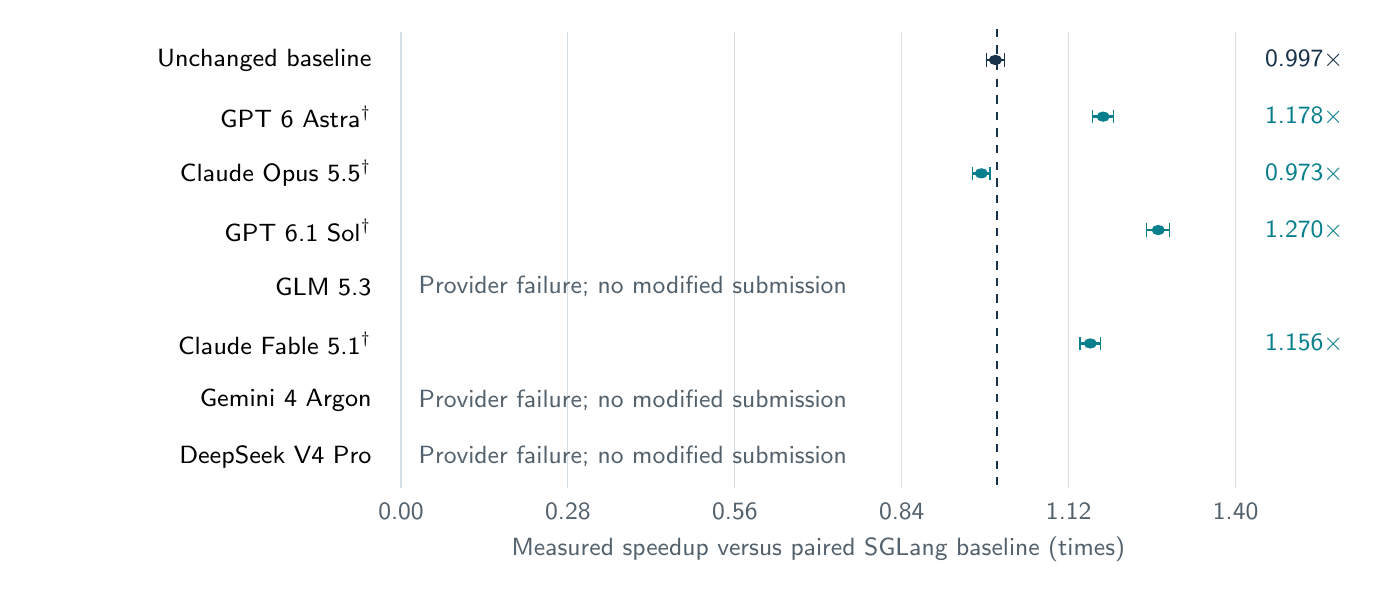
\begin{tikzpicture}[x=1cm,y=.72cm,font=\sffamily\small]
\draw[grid] (0.0000,.5)--(0.0000,-7.5500);
\node[below,text=muted] at (0.0000,-7.6500) {0.00};
\draw[grid] (2.1200,.5)--(2.1200,-7.5500);
\node[below,text=muted] at (2.1200,-7.6500) {0.28};
\draw[grid] (4.2400,.5)--(4.2400,-7.5500);
\node[below,text=muted] at (4.2400,-7.6500) {0.56};
\draw[grid] (6.3600,.5)--(6.3600,-7.5500);
\node[below,text=muted] at (6.3600,-7.6500) {0.84};
\draw[grid] (8.4800,.5)--(8.4800,-7.5500);
\node[below,text=muted] at (8.4800,-7.6500) {1.12};
\draw[grid] (10.6000,.5)--(10.6000,-7.5500);
\node[below,text=muted] at (10.6000,-7.6500) {1.40};
\draw[navy,dashed,thick] (7.5714,.55)--(7.5714,-7.5500);
\node[anchor=east,text width=4.25cm,align=right] at (-.25, 0) {Unchanged baseline};
\draw[navy,line width=1pt] (7.4354, 0)--(7.6619, 0);
\draw[navy] (7.4354,-0.1200)--(7.4354, 0.1200);
\draw[navy] (7.6619,-0.1200)--(7.6619, 0.1200);
\filldraw[draw=navy,fill=navy,line width=1pt] (7.5487, 0) circle (.065);
\node[anchor=west,text=navy] at (10.85, 0) {0.997$\times$};
\node[anchor=east,text width=4.25cm,align=right] at (-.25,-1) {GPT 6 Astra$^{\dagger}$};
\draw[teal,line width=1pt] (8.7834,-1)--(9.0509,-1);
\draw[teal] (8.7834,-1.1200)--(8.7834,-0.8800);
\draw[teal] (9.0509,-1.1200)--(9.0509,-0.8800);
\filldraw[draw=teal,fill=teal,line width=1pt] (8.9171,-1) circle (.065);
\node[anchor=west,text=teal] at (10.85,-1) {1.178$\times$};
\node[anchor=east,text width=4.25cm,align=right] at (-.25,-2) {Claude Opus 5.5$^{\dagger}$};
\draw[teal,line width=1pt] (7.2596,-2)--(7.4807,-2);
\draw[teal] (7.2596,-2.1200)--(7.2596,-1.8800);
\draw[teal] (7.4807,-2.1200)--(7.4807,-1.8800);
\filldraw[draw=teal,fill=teal,line width=1pt] (7.3701,-2) circle (.065);
\node[anchor=west,text=teal] at (10.85,-2) {0.973$\times$};
\node[anchor=east,text width=4.25cm,align=right] at (-.25,-3) {GPT 6.1 Sol$^{\dagger}$};
\draw[teal,line width=1pt] (9.4727,-3)--(9.7612,-3);
\draw[teal] (9.4727,-3.1200)--(9.4727,-2.8800);
\draw[teal] (9.7612,-3.1200)--(9.7612,-2.8800);
\filldraw[draw=teal,fill=teal,line width=1pt] (9.6170,-3) circle (.065);
\node[anchor=west,text=teal] at (10.85,-3) {1.270$\times$};
\node[anchor=east,text width=4.25cm,align=right] at (-.25,-4) {GLM 5.3};
\node[anchor=west,text=muted] at (.1,-4) {Provider failure; no modified submission};
\node[anchor=east,text width=4.25cm,align=right] at (-.25,-5) {Claude Fable 5.1$^{\dagger}$};
\draw[teal,line width=1pt] (8.6227,-5)--(8.8853,-5);
\draw[teal] (8.6227,-5.1200)--(8.6227,-4.8800);
\draw[teal] (8.8853,-5.1200)--(8.8853,-4.8800);
\filldraw[draw=teal,fill=teal,line width=1pt] (8.7540,-5) circle (.065);
\node[anchor=west,text=teal] at (10.85,-5) {1.156$\times$};
\node[anchor=east,text width=4.25cm,align=right] at (-.25,-6) {Gemini 4 Argon};
\node[anchor=west,text=muted] at (.1,-6) {Provider failure; no modified submission};
\node[anchor=east,text width=4.25cm,align=right] at (-.25,-7) {DeepSeek V4 Pro};
\node[anchor=west,text=muted] at (.1,-7) {Provider failure; no modified submission};
\node[below,text=muted] at (5.3,-8.2400) {Measured speedup versus paired SGLang baseline (times)};
\end{tikzpicture}
\caption{Correctness-gated observations and reported 95\% timing intervals. Filled model points represent individually reviewed current-rule-eligible artifacts, not an overall seven-model ranking. A dagger marks a frozen-TASK precision difference. The dashed line is 1$\times$. Intervals describe kernel timing, not variation across agent trials. Missing timings are not zero.}
\end{figure}

\begin{figure}[H]\centering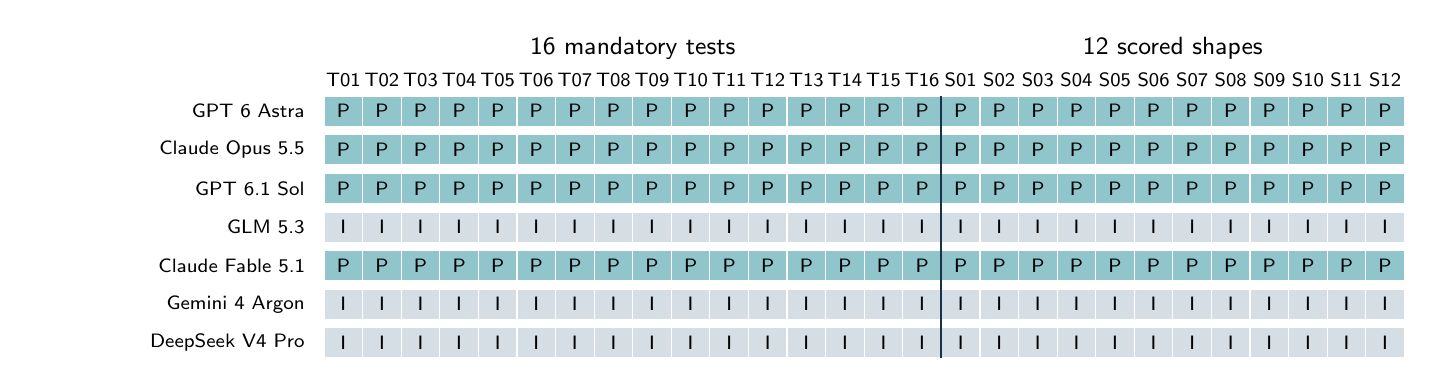
\begin{tikzpicture}[x=.49cm,y=.49cm,font=\sffamily\scriptsize]
\node[above] at (0.50,.4) {T01};
\node[above] at (1.50,.4) {T02};
\node[above] at (2.50,.4) {T03};
\node[above] at (3.50,.4) {T04};
\node[above] at (4.50,.4) {T05};
\node[above] at (5.50,.4) {T06};
\node[above] at (6.50,.4) {T07};
\node[above] at (7.50,.4) {T08};
\node[above] at (8.50,.4) {T09};
\node[above] at (9.50,.4) {T10};
\node[above] at (10.50,.4) {T11};
\node[above] at (11.50,.4) {T12};
\node[above] at (12.50,.4) {T13};
\node[above] at (13.50,.4) {T14};
\node[above] at (14.50,.4) {T15};
\node[above] at (15.50,.4) {T16};
\node[above] at (16.50,.4) {S01};
\node[above] at (17.50,.4) {S02};
\node[above] at (18.50,.4) {S03};
\node[above] at (19.50,.4) {S04};
\node[above] at (20.50,.4) {S05};
\node[above] at (21.50,.4) {S06};
\node[above] at (22.50,.4) {S07};
\node[above] at (23.50,.4) {S08};
\node[above] at (24.50,.4) {S09};
\node[above] at (25.50,.4) {S10};
\node[above] at (26.50,.4) {S11};
\node[above] at (27.50,.4) {S12};
\node[anchor=east,text width=3.4cm,align=right] at (-.25, 0) {GPT 6 Astra};
\filldraw[fill=teal!45,draw=white,line width=.4pt] (0,-0.39) rectangle (1, 0.39);
\node at (0.5, 0) {P};
\filldraw[fill=teal!45,draw=white,line width=.4pt] (1,-0.39) rectangle (2, 0.39);
\node at (1.5, 0) {P};
\filldraw[fill=teal!45,draw=white,line width=.4pt] (2,-0.39) rectangle (3, 0.39);
\node at (2.5, 0) {P};
\filldraw[fill=teal!45,draw=white,line width=.4pt] (3,-0.39) rectangle (4, 0.39);
\node at (3.5, 0) {P};
\filldraw[fill=teal!45,draw=white,line width=.4pt] (4,-0.39) rectangle (5, 0.39);
\node at (4.5, 0) {P};
\filldraw[fill=teal!45,draw=white,line width=.4pt] (5,-0.39) rectangle (6, 0.39);
\node at (5.5, 0) {P};
\filldraw[fill=teal!45,draw=white,line width=.4pt] (6,-0.39) rectangle (7, 0.39);
\node at (6.5, 0) {P};
\filldraw[fill=teal!45,draw=white,line width=.4pt] (7,-0.39) rectangle (8, 0.39);
\node at (7.5, 0) {P};
\filldraw[fill=teal!45,draw=white,line width=.4pt] (8,-0.39) rectangle (9, 0.39);
\node at (8.5, 0) {P};
\filldraw[fill=teal!45,draw=white,line width=.4pt] (9,-0.39) rectangle (10, 0.39);
\node at (9.5, 0) {P};
\filldraw[fill=teal!45,draw=white,line width=.4pt] (10,-0.39) rectangle (11, 0.39);
\node at (10.5, 0) {P};
\filldraw[fill=teal!45,draw=white,line width=.4pt] (11,-0.39) rectangle (12, 0.39);
\node at (11.5, 0) {P};
\filldraw[fill=teal!45,draw=white,line width=.4pt] (12,-0.39) rectangle (13, 0.39);
\node at (12.5, 0) {P};
\filldraw[fill=teal!45,draw=white,line width=.4pt] (13,-0.39) rectangle (14, 0.39);
\node at (13.5, 0) {P};
\filldraw[fill=teal!45,draw=white,line width=.4pt] (14,-0.39) rectangle (15, 0.39);
\node at (14.5, 0) {P};
\filldraw[fill=teal!45,draw=white,line width=.4pt] (15,-0.39) rectangle (16, 0.39);
\node at (15.5, 0) {P};
\filldraw[fill=teal!45,draw=white,line width=.4pt] (16,-0.39) rectangle (17, 0.39);
\node at (16.5, 0) {P};
\filldraw[fill=teal!45,draw=white,line width=.4pt] (17,-0.39) rectangle (18, 0.39);
\node at (17.5, 0) {P};
\filldraw[fill=teal!45,draw=white,line width=.4pt] (18,-0.39) rectangle (19, 0.39);
\node at (18.5, 0) {P};
\filldraw[fill=teal!45,draw=white,line width=.4pt] (19,-0.39) rectangle (20, 0.39);
\node at (19.5, 0) {P};
\filldraw[fill=teal!45,draw=white,line width=.4pt] (20,-0.39) rectangle (21, 0.39);
\node at (20.5, 0) {P};
\filldraw[fill=teal!45,draw=white,line width=.4pt] (21,-0.39) rectangle (22, 0.39);
\node at (21.5, 0) {P};
\filldraw[fill=teal!45,draw=white,line width=.4pt] (22,-0.39) rectangle (23, 0.39);
\node at (22.5, 0) {P};
\filldraw[fill=teal!45,draw=white,line width=.4pt] (23,-0.39) rectangle (24, 0.39);
\node at (23.5, 0) {P};
\filldraw[fill=teal!45,draw=white,line width=.4pt] (24,-0.39) rectangle (25, 0.39);
\node at (24.5, 0) {P};
\filldraw[fill=teal!45,draw=white,line width=.4pt] (25,-0.39) rectangle (26, 0.39);
\node at (25.5, 0) {P};
\filldraw[fill=teal!45,draw=white,line width=.4pt] (26,-0.39) rectangle (27, 0.39);
\node at (26.5, 0) {P};
\filldraw[fill=teal!45,draw=white,line width=.4pt] (27,-0.39) rectangle (28, 0.39);
\node at (27.5, 0) {P};
\node[anchor=east,text width=3.4cm,align=right] at (-.25,-1) {Claude Opus 5.5};
\filldraw[fill=teal!45,draw=white,line width=.4pt] (0,-1.39) rectangle (1,-0.61);
\node at (0.5,-1) {P};
\filldraw[fill=teal!45,draw=white,line width=.4pt] (1,-1.39) rectangle (2,-0.61);
\node at (1.5,-1) {P};
\filldraw[fill=teal!45,draw=white,line width=.4pt] (2,-1.39) rectangle (3,-0.61);
\node at (2.5,-1) {P};
\filldraw[fill=teal!45,draw=white,line width=.4pt] (3,-1.39) rectangle (4,-0.61);
\node at (3.5,-1) {P};
\filldraw[fill=teal!45,draw=white,line width=.4pt] (4,-1.39) rectangle (5,-0.61);
\node at (4.5,-1) {P};
\filldraw[fill=teal!45,draw=white,line width=.4pt] (5,-1.39) rectangle (6,-0.61);
\node at (5.5,-1) {P};
\filldraw[fill=teal!45,draw=white,line width=.4pt] (6,-1.39) rectangle (7,-0.61);
\node at (6.5,-1) {P};
\filldraw[fill=teal!45,draw=white,line width=.4pt] (7,-1.39) rectangle (8,-0.61);
\node at (7.5,-1) {P};
\filldraw[fill=teal!45,draw=white,line width=.4pt] (8,-1.39) rectangle (9,-0.61);
\node at (8.5,-1) {P};
\filldraw[fill=teal!45,draw=white,line width=.4pt] (9,-1.39) rectangle (10,-0.61);
\node at (9.5,-1) {P};
\filldraw[fill=teal!45,draw=white,line width=.4pt] (10,-1.39) rectangle (11,-0.61);
\node at (10.5,-1) {P};
\filldraw[fill=teal!45,draw=white,line width=.4pt] (11,-1.39) rectangle (12,-0.61);
\node at (11.5,-1) {P};
\filldraw[fill=teal!45,draw=white,line width=.4pt] (12,-1.39) rectangle (13,-0.61);
\node at (12.5,-1) {P};
\filldraw[fill=teal!45,draw=white,line width=.4pt] (13,-1.39) rectangle (14,-0.61);
\node at (13.5,-1) {P};
\filldraw[fill=teal!45,draw=white,line width=.4pt] (14,-1.39) rectangle (15,-0.61);
\node at (14.5,-1) {P};
\filldraw[fill=teal!45,draw=white,line width=.4pt] (15,-1.39) rectangle (16,-0.61);
\node at (15.5,-1) {P};
\filldraw[fill=teal!45,draw=white,line width=.4pt] (16,-1.39) rectangle (17,-0.61);
\node at (16.5,-1) {P};
\filldraw[fill=teal!45,draw=white,line width=.4pt] (17,-1.39) rectangle (18,-0.61);
\node at (17.5,-1) {P};
\filldraw[fill=teal!45,draw=white,line width=.4pt] (18,-1.39) rectangle (19,-0.61);
\node at (18.5,-1) {P};
\filldraw[fill=teal!45,draw=white,line width=.4pt] (19,-1.39) rectangle (20,-0.61);
\node at (19.5,-1) {P};
\filldraw[fill=teal!45,draw=white,line width=.4pt] (20,-1.39) rectangle (21,-0.61);
\node at (20.5,-1) {P};
\filldraw[fill=teal!45,draw=white,line width=.4pt] (21,-1.39) rectangle (22,-0.61);
\node at (21.5,-1) {P};
\filldraw[fill=teal!45,draw=white,line width=.4pt] (22,-1.39) rectangle (23,-0.61);
\node at (22.5,-1) {P};
\filldraw[fill=teal!45,draw=white,line width=.4pt] (23,-1.39) rectangle (24,-0.61);
\node at (23.5,-1) {P};
\filldraw[fill=teal!45,draw=white,line width=.4pt] (24,-1.39) rectangle (25,-0.61);
\node at (24.5,-1) {P};
\filldraw[fill=teal!45,draw=white,line width=.4pt] (25,-1.39) rectangle (26,-0.61);
\node at (25.5,-1) {P};
\filldraw[fill=teal!45,draw=white,line width=.4pt] (26,-1.39) rectangle (27,-0.61);
\node at (26.5,-1) {P};
\filldraw[fill=teal!45,draw=white,line width=.4pt] (27,-1.39) rectangle (28,-0.61);
\node at (27.5,-1) {P};
\node[anchor=east,text width=3.4cm,align=right] at (-.25,-2) {GPT 6.1 Sol};
\filldraw[fill=teal!45,draw=white,line width=.4pt] (0,-2.39) rectangle (1,-1.61);
\node at (0.5,-2) {P};
\filldraw[fill=teal!45,draw=white,line width=.4pt] (1,-2.39) rectangle (2,-1.61);
\node at (1.5,-2) {P};
\filldraw[fill=teal!45,draw=white,line width=.4pt] (2,-2.39) rectangle (3,-1.61);
\node at (2.5,-2) {P};
\filldraw[fill=teal!45,draw=white,line width=.4pt] (3,-2.39) rectangle (4,-1.61);
\node at (3.5,-2) {P};
\filldraw[fill=teal!45,draw=white,line width=.4pt] (4,-2.39) rectangle (5,-1.61);
\node at (4.5,-2) {P};
\filldraw[fill=teal!45,draw=white,line width=.4pt] (5,-2.39) rectangle (6,-1.61);
\node at (5.5,-2) {P};
\filldraw[fill=teal!45,draw=white,line width=.4pt] (6,-2.39) rectangle (7,-1.61);
\node at (6.5,-2) {P};
\filldraw[fill=teal!45,draw=white,line width=.4pt] (7,-2.39) rectangle (8,-1.61);
\node at (7.5,-2) {P};
\filldraw[fill=teal!45,draw=white,line width=.4pt] (8,-2.39) rectangle (9,-1.61);
\node at (8.5,-2) {P};
\filldraw[fill=teal!45,draw=white,line width=.4pt] (9,-2.39) rectangle (10,-1.61);
\node at (9.5,-2) {P};
\filldraw[fill=teal!45,draw=white,line width=.4pt] (10,-2.39) rectangle (11,-1.61);
\node at (10.5,-2) {P};
\filldraw[fill=teal!45,draw=white,line width=.4pt] (11,-2.39) rectangle (12,-1.61);
\node at (11.5,-2) {P};
\filldraw[fill=teal!45,draw=white,line width=.4pt] (12,-2.39) rectangle (13,-1.61);
\node at (12.5,-2) {P};
\filldraw[fill=teal!45,draw=white,line width=.4pt] (13,-2.39) rectangle (14,-1.61);
\node at (13.5,-2) {P};
\filldraw[fill=teal!45,draw=white,line width=.4pt] (14,-2.39) rectangle (15,-1.61);
\node at (14.5,-2) {P};
\filldraw[fill=teal!45,draw=white,line width=.4pt] (15,-2.39) rectangle (16,-1.61);
\node at (15.5,-2) {P};
\filldraw[fill=teal!45,draw=white,line width=.4pt] (16,-2.39) rectangle (17,-1.61);
\node at (16.5,-2) {P};
\filldraw[fill=teal!45,draw=white,line width=.4pt] (17,-2.39) rectangle (18,-1.61);
\node at (17.5,-2) {P};
\filldraw[fill=teal!45,draw=white,line width=.4pt] (18,-2.39) rectangle (19,-1.61);
\node at (18.5,-2) {P};
\filldraw[fill=teal!45,draw=white,line width=.4pt] (19,-2.39) rectangle (20,-1.61);
\node at (19.5,-2) {P};
\filldraw[fill=teal!45,draw=white,line width=.4pt] (20,-2.39) rectangle (21,-1.61);
\node at (20.5,-2) {P};
\filldraw[fill=teal!45,draw=white,line width=.4pt] (21,-2.39) rectangle (22,-1.61);
\node at (21.5,-2) {P};
\filldraw[fill=teal!45,draw=white,line width=.4pt] (22,-2.39) rectangle (23,-1.61);
\node at (22.5,-2) {P};
\filldraw[fill=teal!45,draw=white,line width=.4pt] (23,-2.39) rectangle (24,-1.61);
\node at (23.5,-2) {P};
\filldraw[fill=teal!45,draw=white,line width=.4pt] (24,-2.39) rectangle (25,-1.61);
\node at (24.5,-2) {P};
\filldraw[fill=teal!45,draw=white,line width=.4pt] (25,-2.39) rectangle (26,-1.61);
\node at (25.5,-2) {P};
\filldraw[fill=teal!45,draw=white,line width=.4pt] (26,-2.39) rectangle (27,-1.61);
\node at (26.5,-2) {P};
\filldraw[fill=teal!45,draw=white,line width=.4pt] (27,-2.39) rectangle (28,-1.61);
\node at (27.5,-2) {P};
\node[anchor=east,text width=3.4cm,align=right] at (-.25,-3) {GLM 5.3};
\filldraw[fill=grid,draw=white,line width=.4pt] (0,-3.39) rectangle (1,-2.61);
\node at (0.5,-3) {I};
\filldraw[fill=grid,draw=white,line width=.4pt] (1,-3.39) rectangle (2,-2.61);
\node at (1.5,-3) {I};
\filldraw[fill=grid,draw=white,line width=.4pt] (2,-3.39) rectangle (3,-2.61);
\node at (2.5,-3) {I};
\filldraw[fill=grid,draw=white,line width=.4pt] (3,-3.39) rectangle (4,-2.61);
\node at (3.5,-3) {I};
\filldraw[fill=grid,draw=white,line width=.4pt] (4,-3.39) rectangle (5,-2.61);
\node at (4.5,-3) {I};
\filldraw[fill=grid,draw=white,line width=.4pt] (5,-3.39) rectangle (6,-2.61);
\node at (5.5,-3) {I};
\filldraw[fill=grid,draw=white,line width=.4pt] (6,-3.39) rectangle (7,-2.61);
\node at (6.5,-3) {I};
\filldraw[fill=grid,draw=white,line width=.4pt] (7,-3.39) rectangle (8,-2.61);
\node at (7.5,-3) {I};
\filldraw[fill=grid,draw=white,line width=.4pt] (8,-3.39) rectangle (9,-2.61);
\node at (8.5,-3) {I};
\filldraw[fill=grid,draw=white,line width=.4pt] (9,-3.39) rectangle (10,-2.61);
\node at (9.5,-3) {I};
\filldraw[fill=grid,draw=white,line width=.4pt] (10,-3.39) rectangle (11,-2.61);
\node at (10.5,-3) {I};
\filldraw[fill=grid,draw=white,line width=.4pt] (11,-3.39) rectangle (12,-2.61);
\node at (11.5,-3) {I};
\filldraw[fill=grid,draw=white,line width=.4pt] (12,-3.39) rectangle (13,-2.61);
\node at (12.5,-3) {I};
\filldraw[fill=grid,draw=white,line width=.4pt] (13,-3.39) rectangle (14,-2.61);
\node at (13.5,-3) {I};
\filldraw[fill=grid,draw=white,line width=.4pt] (14,-3.39) rectangle (15,-2.61);
\node at (14.5,-3) {I};
\filldraw[fill=grid,draw=white,line width=.4pt] (15,-3.39) rectangle (16,-2.61);
\node at (15.5,-3) {I};
\filldraw[fill=grid,draw=white,line width=.4pt] (16,-3.39) rectangle (17,-2.61);
\node at (16.5,-3) {I};
\filldraw[fill=grid,draw=white,line width=.4pt] (17,-3.39) rectangle (18,-2.61);
\node at (17.5,-3) {I};
\filldraw[fill=grid,draw=white,line width=.4pt] (18,-3.39) rectangle (19,-2.61);
\node at (18.5,-3) {I};
\filldraw[fill=grid,draw=white,line width=.4pt] (19,-3.39) rectangle (20,-2.61);
\node at (19.5,-3) {I};
\filldraw[fill=grid,draw=white,line width=.4pt] (20,-3.39) rectangle (21,-2.61);
\node at (20.5,-3) {I};
\filldraw[fill=grid,draw=white,line width=.4pt] (21,-3.39) rectangle (22,-2.61);
\node at (21.5,-3) {I};
\filldraw[fill=grid,draw=white,line width=.4pt] (22,-3.39) rectangle (23,-2.61);
\node at (22.5,-3) {I};
\filldraw[fill=grid,draw=white,line width=.4pt] (23,-3.39) rectangle (24,-2.61);
\node at (23.5,-3) {I};
\filldraw[fill=grid,draw=white,line width=.4pt] (24,-3.39) rectangle (25,-2.61);
\node at (24.5,-3) {I};
\filldraw[fill=grid,draw=white,line width=.4pt] (25,-3.39) rectangle (26,-2.61);
\node at (25.5,-3) {I};
\filldraw[fill=grid,draw=white,line width=.4pt] (26,-3.39) rectangle (27,-2.61);
\node at (26.5,-3) {I};
\filldraw[fill=grid,draw=white,line width=.4pt] (27,-3.39) rectangle (28,-2.61);
\node at (27.5,-3) {I};
\node[anchor=east,text width=3.4cm,align=right] at (-.25,-4) {Claude Fable 5.1};
\filldraw[fill=teal!45,draw=white,line width=.4pt] (0,-4.39) rectangle (1,-3.61);
\node at (0.5,-4) {P};
\filldraw[fill=teal!45,draw=white,line width=.4pt] (1,-4.39) rectangle (2,-3.61);
\node at (1.5,-4) {P};
\filldraw[fill=teal!45,draw=white,line width=.4pt] (2,-4.39) rectangle (3,-3.61);
\node at (2.5,-4) {P};
\filldraw[fill=teal!45,draw=white,line width=.4pt] (3,-4.39) rectangle (4,-3.61);
\node at (3.5,-4) {P};
\filldraw[fill=teal!45,draw=white,line width=.4pt] (4,-4.39) rectangle (5,-3.61);
\node at (4.5,-4) {P};
\filldraw[fill=teal!45,draw=white,line width=.4pt] (5,-4.39) rectangle (6,-3.61);
\node at (5.5,-4) {P};
\filldraw[fill=teal!45,draw=white,line width=.4pt] (6,-4.39) rectangle (7,-3.61);
\node at (6.5,-4) {P};
\filldraw[fill=teal!45,draw=white,line width=.4pt] (7,-4.39) rectangle (8,-3.61);
\node at (7.5,-4) {P};
\filldraw[fill=teal!45,draw=white,line width=.4pt] (8,-4.39) rectangle (9,-3.61);
\node at (8.5,-4) {P};
\filldraw[fill=teal!45,draw=white,line width=.4pt] (9,-4.39) rectangle (10,-3.61);
\node at (9.5,-4) {P};
\filldraw[fill=teal!45,draw=white,line width=.4pt] (10,-4.39) rectangle (11,-3.61);
\node at (10.5,-4) {P};
\filldraw[fill=teal!45,draw=white,line width=.4pt] (11,-4.39) rectangle (12,-3.61);
\node at (11.5,-4) {P};
\filldraw[fill=teal!45,draw=white,line width=.4pt] (12,-4.39) rectangle (13,-3.61);
\node at (12.5,-4) {P};
\filldraw[fill=teal!45,draw=white,line width=.4pt] (13,-4.39) rectangle (14,-3.61);
\node at (13.5,-4) {P};
\filldraw[fill=teal!45,draw=white,line width=.4pt] (14,-4.39) rectangle (15,-3.61);
\node at (14.5,-4) {P};
\filldraw[fill=teal!45,draw=white,line width=.4pt] (15,-4.39) rectangle (16,-3.61);
\node at (15.5,-4) {P};
\filldraw[fill=teal!45,draw=white,line width=.4pt] (16,-4.39) rectangle (17,-3.61);
\node at (16.5,-4) {P};
\filldraw[fill=teal!45,draw=white,line width=.4pt] (17,-4.39) rectangle (18,-3.61);
\node at (17.5,-4) {P};
\filldraw[fill=teal!45,draw=white,line width=.4pt] (18,-4.39) rectangle (19,-3.61);
\node at (18.5,-4) {P};
\filldraw[fill=teal!45,draw=white,line width=.4pt] (19,-4.39) rectangle (20,-3.61);
\node at (19.5,-4) {P};
\filldraw[fill=teal!45,draw=white,line width=.4pt] (20,-4.39) rectangle (21,-3.61);
\node at (20.5,-4) {P};
\filldraw[fill=teal!45,draw=white,line width=.4pt] (21,-4.39) rectangle (22,-3.61);
\node at (21.5,-4) {P};
\filldraw[fill=teal!45,draw=white,line width=.4pt] (22,-4.39) rectangle (23,-3.61);
\node at (22.5,-4) {P};
\filldraw[fill=teal!45,draw=white,line width=.4pt] (23,-4.39) rectangle (24,-3.61);
\node at (23.5,-4) {P};
\filldraw[fill=teal!45,draw=white,line width=.4pt] (24,-4.39) rectangle (25,-3.61);
\node at (24.5,-4) {P};
\filldraw[fill=teal!45,draw=white,line width=.4pt] (25,-4.39) rectangle (26,-3.61);
\node at (25.5,-4) {P};
\filldraw[fill=teal!45,draw=white,line width=.4pt] (26,-4.39) rectangle (27,-3.61);
\node at (26.5,-4) {P};
\filldraw[fill=teal!45,draw=white,line width=.4pt] (27,-4.39) rectangle (28,-3.61);
\node at (27.5,-4) {P};
\node[anchor=east,text width=3.4cm,align=right] at (-.25,-5) {Gemini 4 Argon};
\filldraw[fill=grid,draw=white,line width=.4pt] (0,-5.39) rectangle (1,-4.61);
\node at (0.5,-5) {I};
\filldraw[fill=grid,draw=white,line width=.4pt] (1,-5.39) rectangle (2,-4.61);
\node at (1.5,-5) {I};
\filldraw[fill=grid,draw=white,line width=.4pt] (2,-5.39) rectangle (3,-4.61);
\node at (2.5,-5) {I};
\filldraw[fill=grid,draw=white,line width=.4pt] (3,-5.39) rectangle (4,-4.61);
\node at (3.5,-5) {I};
\filldraw[fill=grid,draw=white,line width=.4pt] (4,-5.39) rectangle (5,-4.61);
\node at (4.5,-5) {I};
\filldraw[fill=grid,draw=white,line width=.4pt] (5,-5.39) rectangle (6,-4.61);
\node at (5.5,-5) {I};
\filldraw[fill=grid,draw=white,line width=.4pt] (6,-5.39) rectangle (7,-4.61);
\node at (6.5,-5) {I};
\filldraw[fill=grid,draw=white,line width=.4pt] (7,-5.39) rectangle (8,-4.61);
\node at (7.5,-5) {I};
\filldraw[fill=grid,draw=white,line width=.4pt] (8,-5.39) rectangle (9,-4.61);
\node at (8.5,-5) {I};
\filldraw[fill=grid,draw=white,line width=.4pt] (9,-5.39) rectangle (10,-4.61);
\node at (9.5,-5) {I};
\filldraw[fill=grid,draw=white,line width=.4pt] (10,-5.39) rectangle (11,-4.61);
\node at (10.5,-5) {I};
\filldraw[fill=grid,draw=white,line width=.4pt] (11,-5.39) rectangle (12,-4.61);
\node at (11.5,-5) {I};
\filldraw[fill=grid,draw=white,line width=.4pt] (12,-5.39) rectangle (13,-4.61);
\node at (12.5,-5) {I};
\filldraw[fill=grid,draw=white,line width=.4pt] (13,-5.39) rectangle (14,-4.61);
\node at (13.5,-5) {I};
\filldraw[fill=grid,draw=white,line width=.4pt] (14,-5.39) rectangle (15,-4.61);
\node at (14.5,-5) {I};
\filldraw[fill=grid,draw=white,line width=.4pt] (15,-5.39) rectangle (16,-4.61);
\node at (15.5,-5) {I};
\filldraw[fill=grid,draw=white,line width=.4pt] (16,-5.39) rectangle (17,-4.61);
\node at (16.5,-5) {I};
\filldraw[fill=grid,draw=white,line width=.4pt] (17,-5.39) rectangle (18,-4.61);
\node at (17.5,-5) {I};
\filldraw[fill=grid,draw=white,line width=.4pt] (18,-5.39) rectangle (19,-4.61);
\node at (18.5,-5) {I};
\filldraw[fill=grid,draw=white,line width=.4pt] (19,-5.39) rectangle (20,-4.61);
\node at (19.5,-5) {I};
\filldraw[fill=grid,draw=white,line width=.4pt] (20,-5.39) rectangle (21,-4.61);
\node at (20.5,-5) {I};
\filldraw[fill=grid,draw=white,line width=.4pt] (21,-5.39) rectangle (22,-4.61);
\node at (21.5,-5) {I};
\filldraw[fill=grid,draw=white,line width=.4pt] (22,-5.39) rectangle (23,-4.61);
\node at (22.5,-5) {I};
\filldraw[fill=grid,draw=white,line width=.4pt] (23,-5.39) rectangle (24,-4.61);
\node at (23.5,-5) {I};
\filldraw[fill=grid,draw=white,line width=.4pt] (24,-5.39) rectangle (25,-4.61);
\node at (24.5,-5) {I};
\filldraw[fill=grid,draw=white,line width=.4pt] (25,-5.39) rectangle (26,-4.61);
\node at (25.5,-5) {I};
\filldraw[fill=grid,draw=white,line width=.4pt] (26,-5.39) rectangle (27,-4.61);
\node at (26.5,-5) {I};
\filldraw[fill=grid,draw=white,line width=.4pt] (27,-5.39) rectangle (28,-4.61);
\node at (27.5,-5) {I};
\node[anchor=east,text width=3.4cm,align=right] at (-.25,-6) {DeepSeek V4 Pro};
\filldraw[fill=grid,draw=white,line width=.4pt] (0,-6.39) rectangle (1,-5.61);
\node at (0.5,-6) {I};
\filldraw[fill=grid,draw=white,line width=.4pt] (1,-6.39) rectangle (2,-5.61);
\node at (1.5,-6) {I};
\filldraw[fill=grid,draw=white,line width=.4pt] (2,-6.39) rectangle (3,-5.61);
\node at (2.5,-6) {I};
\filldraw[fill=grid,draw=white,line width=.4pt] (3,-6.39) rectangle (4,-5.61);
\node at (3.5,-6) {I};
\filldraw[fill=grid,draw=white,line width=.4pt] (4,-6.39) rectangle (5,-5.61);
\node at (4.5,-6) {I};
\filldraw[fill=grid,draw=white,line width=.4pt] (5,-6.39) rectangle (6,-5.61);
\node at (5.5,-6) {I};
\filldraw[fill=grid,draw=white,line width=.4pt] (6,-6.39) rectangle (7,-5.61);
\node at (6.5,-6) {I};
\filldraw[fill=grid,draw=white,line width=.4pt] (7,-6.39) rectangle (8,-5.61);
\node at (7.5,-6) {I};
\filldraw[fill=grid,draw=white,line width=.4pt] (8,-6.39) rectangle (9,-5.61);
\node at (8.5,-6) {I};
\filldraw[fill=grid,draw=white,line width=.4pt] (9,-6.39) rectangle (10,-5.61);
\node at (9.5,-6) {I};
\filldraw[fill=grid,draw=white,line width=.4pt] (10,-6.39) rectangle (11,-5.61);
\node at (10.5,-6) {I};
\filldraw[fill=grid,draw=white,line width=.4pt] (11,-6.39) rectangle (12,-5.61);
\node at (11.5,-6) {I};
\filldraw[fill=grid,draw=white,line width=.4pt] (12,-6.39) rectangle (13,-5.61);
\node at (12.5,-6) {I};
\filldraw[fill=grid,draw=white,line width=.4pt] (13,-6.39) rectangle (14,-5.61);
\node at (13.5,-6) {I};
\filldraw[fill=grid,draw=white,line width=.4pt] (14,-6.39) rectangle (15,-5.61);
\node at (14.5,-6) {I};
\filldraw[fill=grid,draw=white,line width=.4pt] (15,-6.39) rectangle (16,-5.61);
\node at (15.5,-6) {I};
\filldraw[fill=grid,draw=white,line width=.4pt] (16,-6.39) rectangle (17,-5.61);
\node at (16.5,-6) {I};
\filldraw[fill=grid,draw=white,line width=.4pt] (17,-6.39) rectangle (18,-5.61);
\node at (17.5,-6) {I};
\filldraw[fill=grid,draw=white,line width=.4pt] (18,-6.39) rectangle (19,-5.61);
\node at (18.5,-6) {I};
\filldraw[fill=grid,draw=white,line width=.4pt] (19,-6.39) rectangle (20,-5.61);
\node at (19.5,-6) {I};
\filldraw[fill=grid,draw=white,line width=.4pt] (20,-6.39) rectangle (21,-5.61);
\node at (20.5,-6) {I};
\filldraw[fill=grid,draw=white,line width=.4pt] (21,-6.39) rectangle (22,-5.61);
\node at (21.5,-6) {I};
\filldraw[fill=grid,draw=white,line width=.4pt] (22,-6.39) rectangle (23,-5.61);
\node at (22.5,-6) {I};
\filldraw[fill=grid,draw=white,line width=.4pt] (23,-6.39) rectangle (24,-5.61);
\node at (23.5,-6) {I};
\filldraw[fill=grid,draw=white,line width=.4pt] (24,-6.39) rectangle (25,-5.61);
\node at (24.5,-6) {I};
\filldraw[fill=grid,draw=white,line width=.4pt] (25,-6.39) rectangle (26,-5.61);
\node at (25.5,-6) {I};
\filldraw[fill=grid,draw=white,line width=.4pt] (26,-6.39) rectangle (27,-5.61);
\node at (26.5,-6) {I};
\filldraw[fill=grid,draw=white,line width=.4pt] (27,-6.39) rectangle (28,-5.61);
\node at (27.5,-6) {I};
\draw[navy,thick] (16,.4)--(16,-6.40);
\node[above,font=\sffamily\small] at (8, 1.1) {16 mandatory tests};
\node[above,font=\sffamily\small] at (22, 1.1) {12 scored shapes};
\end{tikzpicture}\caption{All 28 source-level correctness observations. P=passing evaluated candidate; I=passing inherited starter control; F=failed check; dash=not observed. Delivery and source approval are separate from these numerical checks. I cells are not new kernels authored by those models. Mandatory tests do not supply per-shape timing measurements.}\end{figure}

\begin{figure}[H]\centering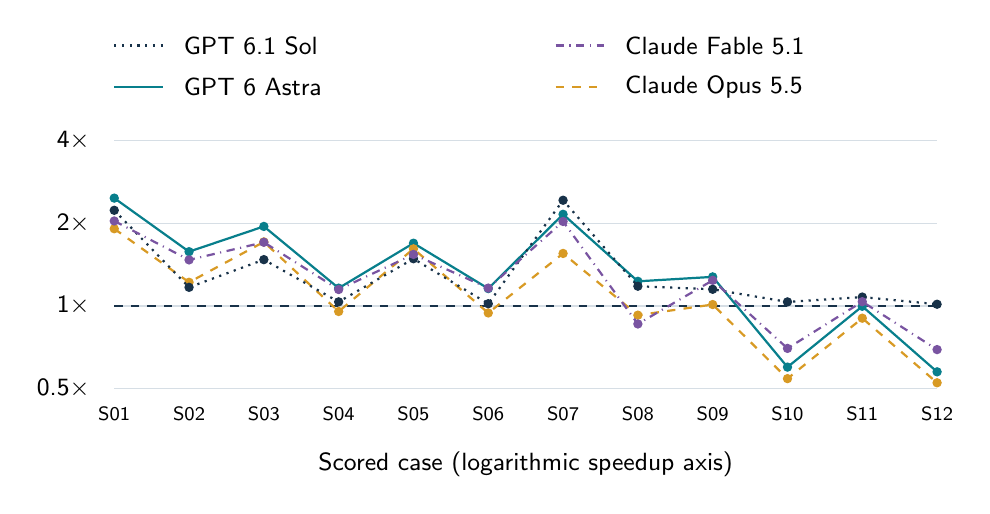
\begin{tikzpicture}[x=.95cm,y=1.05cm,font=\sffamily\small]
\draw[grid] (0,-1)--(11,-1);
\node[anchor=east] at (-.2,-1) {0.5$\times$};
\draw[grid] (0, 0)--(11, 0);
\node[anchor=east] at (-.2, 0) {1$\times$};
\draw[grid] (0, 1)--(11, 1);
\node[anchor=east] at (-.2, 1) {2$\times$};
\draw[grid] (0, 2)--(11, 2);
\node[anchor=east] at (-.2, 2) {4$\times$};
\draw[navy,dashed] (0, 0)--(11, 0);
\node[below,font=\sffamily\scriptsize] at (0,-1.1) {S01};
\node[below,font=\sffamily\scriptsize] at (1,-1.1) {S02};
\node[below,font=\sffamily\scriptsize] at (2,-1.1) {S03};
\node[below,font=\sffamily\scriptsize] at (3,-1.1) {S04};
\node[below,font=\sffamily\scriptsize] at (4,-1.1) {S05};
\node[below,font=\sffamily\scriptsize] at (5,-1.1) {S06};
\node[below,font=\sffamily\scriptsize] at (6,-1.1) {S07};
\node[below,font=\sffamily\scriptsize] at (7,-1.1) {S08};
\node[below,font=\sffamily\scriptsize] at (8,-1.1) {S09};
\node[below,font=\sffamily\scriptsize] at (9,-1.1) {S10};
\node[below,font=\sffamily\scriptsize] at (10,-1.1) {S11};
\node[below,font=\sffamily\scriptsize] at (11,-1.1) {S12};
\draw[teal,solid,thick] (0, 1.30457)--(1, 0.65687)--(2, 0.96223)--(3, 0.21576)--(4, 0.75918)--(5, 0.21051)--(6, 1.10898)--(7, 0.29827)--(8, 0.35197)--(9,-0.73952)--(10,-0.00378)--(11,-0.79646);
\fill[teal] (0, 1.30457) circle (1.7pt);
\fill[teal] (1, 0.65687) circle (1.7pt);
\fill[teal] (2, 0.96223) circle (1.7pt);
\fill[teal] (3, 0.21576) circle (1.7pt);
\fill[teal] (4, 0.75918) circle (1.7pt);
\fill[teal] (5, 0.21051) circle (1.7pt);
\fill[teal] (6, 1.10898) circle (1.7pt);
\fill[teal] (7, 0.29827) circle (1.7pt);
\fill[teal] (8, 0.35197) circle (1.7pt);
\fill[teal] (9,-0.73952) circle (1.7pt);
\fill[teal] (10,-0.00378) circle (1.7pt);
\fill[teal] (11,-0.79646) circle (1.7pt);
\draw[teal,solid,thick] (0.0, 2.65)--(0.65, 2.65);
\node[anchor=west] at (0.8, 2.65) {GPT 6 Astra};
\draw[gold,dashed,thick] (0, 0.93413)--(1, 0.28657)--(2, 0.77492)--(3,-0.06666)--(4, 0.69133)--(5,-0.08455)--(6, 0.63538)--(7,-0.11113)--(8, 0.01740)--(9,-0.87878)--(10,-0.14780)--(11,-0.92890);
\fill[gold] (0, 0.93413) circle (1.7pt);
\fill[gold] (1, 0.28657) circle (1.7pt);
\fill[gold] (2, 0.77492) circle (1.7pt);
\fill[gold] (3,-0.06666) circle (1.7pt);
\fill[gold] (4, 0.69133) circle (1.7pt);
\fill[gold] (5,-0.08455) circle (1.7pt);
\fill[gold] (6, 0.63538) circle (1.7pt);
\fill[gold] (7,-0.11113) circle (1.7pt);
\fill[gold] (8, 0.01740) circle (1.7pt);
\fill[gold] (9,-0.87878) circle (1.7pt);
\fill[gold] (10,-0.14780) circle (1.7pt);
\fill[gold] (11,-0.92890) circle (1.7pt);
\draw[gold,dashed,thick] (5.9, 2.65)--(6.550000000000001, 2.65);
\node[anchor=west] at (6.7, 2.65) {Claude Opus 5.5};
\draw[navy,dotted,thick] (0, 1.15724)--(1, 0.22561)--(2, 0.56060)--(3, 0.04992)--(4, 0.57140)--(5, 0.02716)--(6, 1.27868)--(7, 0.23906)--(8, 0.20183)--(9, 0.04941)--(10, 0.10780)--(11, 0.02116);
\fill[navy] (0, 1.15724) circle (1.7pt);
\fill[navy] (1, 0.22561) circle (1.7pt);
\fill[navy] (2, 0.56060) circle (1.7pt);
\fill[navy] (3, 0.04992) circle (1.7pt);
\fill[navy] (4, 0.57140) circle (1.7pt);
\fill[navy] (5, 0.02716) circle (1.7pt);
\fill[navy] (6, 1.27868) circle (1.7pt);
\fill[navy] (7, 0.23906) circle (1.7pt);
\fill[navy] (8, 0.20183) circle (1.7pt);
\fill[navy] (9, 0.04941) circle (1.7pt);
\fill[navy] (10, 0.10780) circle (1.7pt);
\fill[navy] (11, 0.02116) circle (1.7pt);
\draw[navy,dotted,thick] (0.0, 3.15)--(0.65, 3.15);
\node[anchor=west] at (0.8, 3.15) {GPT 6.1 Sol};
\draw[purple,dashdotted,thick] (0, 1.02824)--(1, 0.55738)--(2, 0.77061)--(3, 0.19881)--(4, 0.62347)--(5, 0.21606)--(6, 1.02214)--(7,-0.21742)--(8, 0.31032)--(9,-0.51288)--(10, 0.05178)--(11,-0.52757);
\fill[purple] (0, 1.02824) circle (1.7pt);
\fill[purple] (1, 0.55738) circle (1.7pt);
\fill[purple] (2, 0.77061) circle (1.7pt);
\fill[purple] (3, 0.19881) circle (1.7pt);
\fill[purple] (4, 0.62347) circle (1.7pt);
\fill[purple] (5, 0.21606) circle (1.7pt);
\fill[purple] (6, 1.02214) circle (1.7pt);
\fill[purple] (7,-0.21742) circle (1.7pt);
\fill[purple] (8, 0.31032) circle (1.7pt);
\fill[purple] (9,-0.51288) circle (1.7pt);
\fill[purple] (10, 0.05178) circle (1.7pt);
\fill[purple] (11,-0.52757) circle (1.7pt);
\draw[purple,dashdotted,thick] (5.9, 3.15)--(6.550000000000001, 3.15);
\node[anchor=west] at (6.7, 3.15) {Claude Fable 5.1};
\node[below] at (5.5,-1.65) {Scored case (logarithmic speedup axis)};
\end{tikzpicture}\caption{The 12 timed-case speedups for modified delivered candidates only. Adjacent pairs are sliding/full cases for decode B1/B16/B32, then verify B1/B16/B32. Shape-specific regressions remain visible. The overall score is the geometric mean of six weighted load ratios, not an average of these12 points.}\end{figure}

\small\begin{tabularx}{\linewidth}{@{}Xllll@{}}\toprule\textbf{Source} & \textbf{Authoring} & \textbf{A outcome} & \textbf{Current rules} & \textbf{Strict TASK}\\\midrule

GPT 6 Astra & R1 / original & passed & Approved & Differs\\

Claude Opus 5.5 & R1 / original & passed & Approved & Differs\\

GPT 6.1 Sol & R1 / original & passed & Approved & Differs\\

GLM 5.3 & R1 / original & passed & Inherited control & N/A\\

Claude Fable 5.1 & R1 / original & passed & Approved & Differs\\

Gemini 4 Argon & R1 / original & passed & Inherited control & N/A\\

DeepSeek V4 Pro & R2 / B & passed & Inherited control & N/A\\

\bottomrule\end{tabularx}\normalsize

\subsection{The six weighted-load ratios}

\small\begin{tabularx}{\linewidth}{@{}Xrrrrrr@{}}\toprule\textbf{Authored artifact} & D1 & D16 & D32 & V1 & V16 & V32\\\midrule

GPT 6 Astra & 2.083 & 1.320 & 1.238 & 1.729 & 0.715 & 0.634\\

Claude Opus 5.5 & 1.607 & 1.099 & 1.032 & 1.271 & 0.635 & 0.578\\

GPT 6.1 Sol & 1.711 & 1.137 & 1.088 & 1.808 & 1.068 & 1.028\\

Claude Fable 5.1 & 1.808 & 1.270 & 1.223 & 1.404 & 0.810 & 0.748\\

\bottomrule\end{tabularx}\normalsize

D denotes decode and V denotes eight-token verify; the suffix is batch size. Each entry combines sliding/full shapes with 46/16 weights before division. Regressions at individual loads are retained; the overall score is the geometric mean of these six ratios.

Timing intervals describe the resulting kernels on A, conditional on each source and local timing protocol. They do not estimate repeated authoring variation or establish a general model-ability winner.

\section{Authoring lineage and parallel evaluation}

\begin{figure}[H]\centering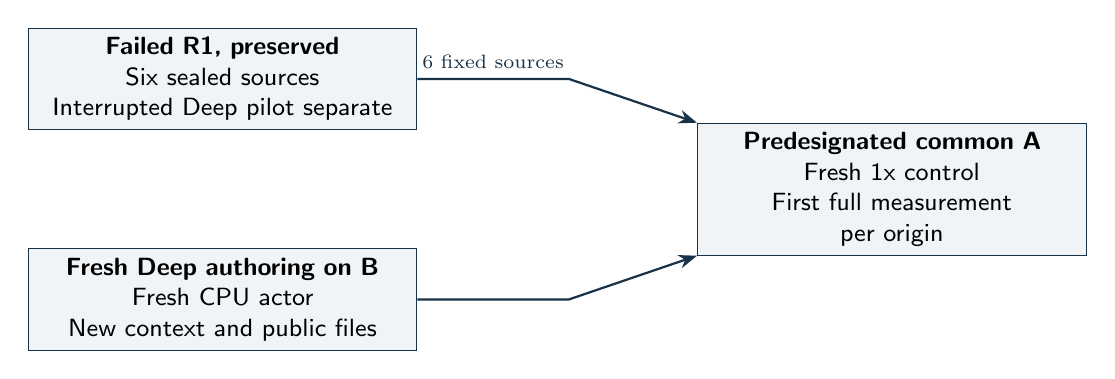
\begin{tikzpicture}[font=\sffamily\small,box/.style={draw=navy,fill=pale,text width=4.7cm,minimum height=1.25cm,align=center},link/.style={-{Stealth},thick,navy}]

\node[box] (old) at (0,.8) {\textbf{Failed R1, preserved}\\Six sealed sources\\Interrupted Deep pilot separate};

\node[box] (new) at (0,-2) {\textbf{Fresh Deep authoring on B}\\Fresh CPU actor\\New context and public files};

\node[box] (common) at (8.5,-.6) {\textbf{Predesignated common A}\\Fresh 1x control\\\mbox{First full measurement}\\per origin};

\draw[link] (old.east)--node[above,font=\scriptsize]{6 fixed sources}(4.4,.8)--(common.north west);

\draw[link] (new.east)--(4.4,-2)--(common.south west);

\end{tikzpicture}\caption{Role A rescoring proceeds in parallel with Deep research/diagnostics on B. No A results or other candidates reach the Deep actor. Different source-authoring conditions remain explicit even though final measurements share one A identity.}\end{figure}

Board roles are recorded without unique hardware or cloud object identifiers. The source-authoring board is distinct from the common-A measurement role; the scientific source hashes remain unchanged.

Deep final queue: 0.000 seconds, outside its research clock. Actual A host-evaluation window: 204.486 seconds. Raw core evaluation wall time is retained separately because it includes this queue. Queue time is not charged again as GPU work; persistent-resource lifetimes are reconciled separately.

\begin{figure}[H]\centering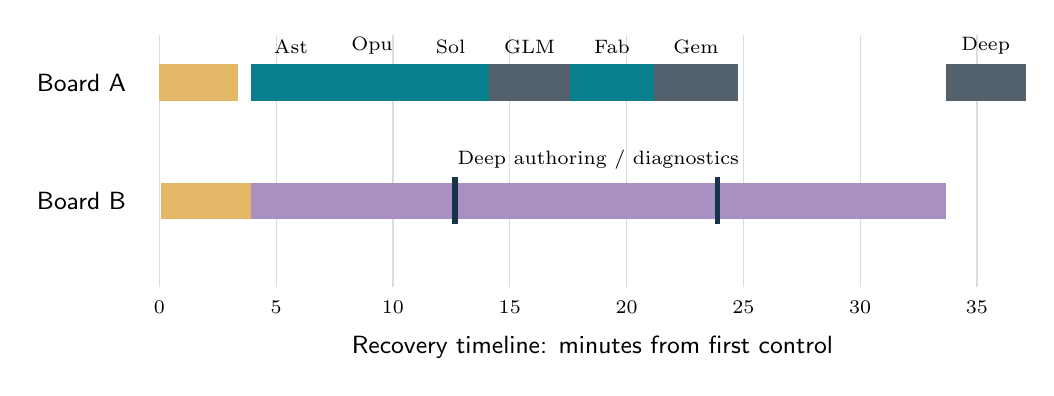
\begin{tikzpicture}[x=1cm,y=1cm,font=\sffamily\small]
\draw[grid] (0.0000,.6)--(0.0000,-2.6);
\node[below,font=\scriptsize] at (0.0000,-2.65) {0};
\draw[grid] (1.4833,.6)--(1.4833,-2.6);
\node[below,font=\scriptsize] at (1.4833,-2.65) {5};
\draw[grid] (2.9667,.6)--(2.9667,-2.6);
\node[below,font=\scriptsize] at (2.9667,-2.65) {10};
\draw[grid] (4.4500,.6)--(4.4500,-2.6);
\node[below,font=\scriptsize] at (4.4500,-2.65) {15};
\draw[grid] (5.9333,.6)--(5.9333,-2.6);
\node[below,font=\scriptsize] at (5.9333,-2.65) {20};
\draw[grid] (7.4167,.6)--(7.4167,-2.6);
\node[below,font=\scriptsize] at (7.4167,-2.65) {25};
\draw[grid] (8.9000,.6)--(8.9000,-2.6);
\node[below,font=\scriptsize] at (8.9000,-2.65) {30};
\draw[grid] (10.3833,.6)--(10.3833,-2.6);
\node[below,font=\scriptsize] at (10.3833,-2.65) {35};
\node[anchor=east] at (-.3, 0) {Board A};
\fill[gold!70] (0.0000,-0.23) rectangle (1.0043, 0.23);
\node[anchor=east] at (-.3,-1.5) {Board B};
\fill[gold!70] (0.0193,-1.73) rectangle (1.1577,-1.27);
\fill[teal] (1.1578,-.23) rectangle (2.1876,.23);
\node[above,font=\scriptsize] at (1.6727,.24) {Ast};
\fill[teal] (2.1876,-.23) rectangle (3.2126,.23);
\node[above,font=\scriptsize] at (2.7001,.24) {Opu};
\fill[teal] (3.2126,-.23) rectangle (4.1869,.23);
\node[above,font=\scriptsize] at (3.6998,.24) {Sol};
\fill[muted] (4.1870,-.23) rectangle (5.2156,.23);
\node[above,font=\scriptsize] at (4.7013,.24) {GLM};
\fill[teal] (5.2156,-.23) rectangle (6.2800,.23);
\node[above,font=\scriptsize] at (5.7478,.24) {Fab};
\fill[muted] (6.2800,-.23) rectangle (7.3477,.23);
\node[above,font=\scriptsize] at (6.8138,.24) {Gem};
\fill[muted] (9.9889,-.23) rectangle (11.0000,.23);
\node[above,font=\scriptsize] at (10.4945,.24) {Deep};
\fill[purple!65] (1.1578,-1.73) rectangle (9.9889,-1.27);
\node[above,font=\scriptsize] at (5.5733,-1.23) {Deep authoring / diagnostics};
\draw[navy,line width=2pt] (3.7548,-1.8)--(3.7548,-1.2);
\draw[navy,line width=2pt] (7.0855,-1.8)--(7.0855,-1.2);
\node[below] at (5.5,-3.1) {Recovery timeline: minutes from first control};
\end{tikzpicture}\caption{Gold: full-suite baseline controls. A then measures the six fixed R1 sources while B supports fresh Deep authoring; the final Deep source is evaluated on A after sealing. Grey A jobs are inherited starter controls, not model performance points. Navy B markers are actual diagnostic starts. Gaps represent setup/idle; queue is outside authoring and is not added as a second GPU phase. The relative chronology omits absolute timestamps and unique resource identities.}\end{figure}

\begin{figure}[H]\centering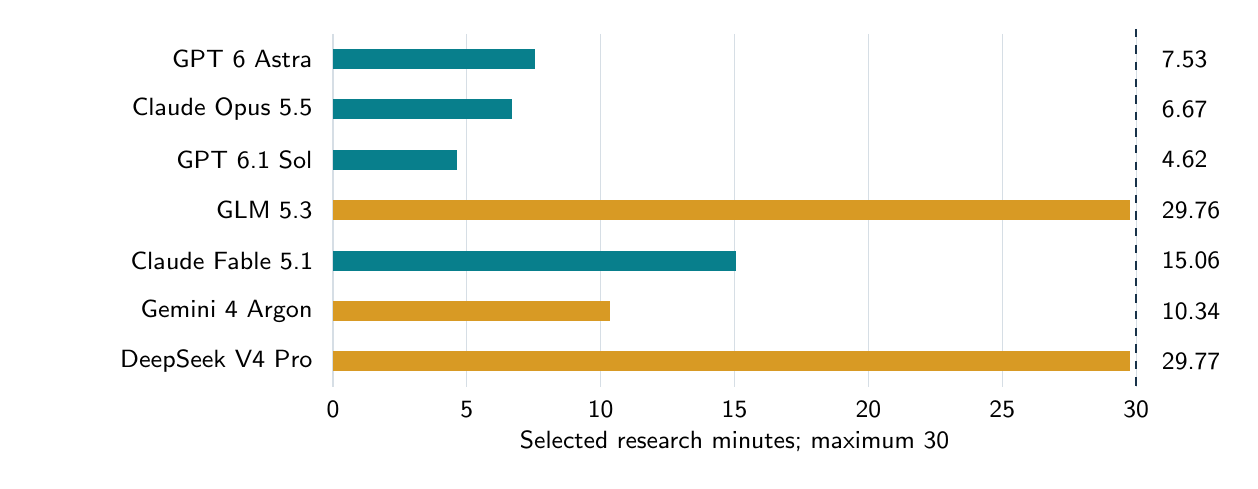
\begin{tikzpicture}[x=.34cm,y=.64cm,font=\sffamily\small]
\draw[grid] (0,.5)--(0,-6.5);
\node[below] at (0,-6.6) {0};
\draw[grid] (5,.5)--(5,-6.5);
\node[below] at (5,-6.6) {5};
\draw[grid] (10,.5)--(10,-6.5);
\node[below] at (10,-6.6) {10};
\draw[grid] (15,.5)--(15,-6.5);
\node[below] at (15,-6.6) {15};
\draw[grid] (20,.5)--(20,-6.5);
\node[below] at (20,-6.6) {20};
\draw[grid] (25,.5)--(25,-6.5);
\node[below] at (25,-6.6) {25};
\draw[grid] (30,.5)--(30,-6.5);
\node[below] at (30,-6.6) {30};
\node[anchor=east,text width=3.5cm,align=right] at (-.4, 0) {GPT 6 Astra};
\fill[teal] (0,-0.2) rectangle (7.53473, 0.2);
\node[anchor=west] at (30.6, 0) {7.53};
\node[anchor=east,text width=3.5cm,align=right] at (-.4,-1) {Claude Opus 5.5};
\fill[teal] (0,-1.2) rectangle (6.67079,-0.8);
\node[anchor=west] at (30.6,-1) {6.67};
\node[anchor=east,text width=3.5cm,align=right] at (-.4,-2) {GPT 6.1 Sol};
\fill[teal] (0,-2.2) rectangle (4.62492,-1.8);
\node[anchor=west] at (30.6,-2) {4.62};
\node[anchor=east,text width=3.5cm,align=right] at (-.4,-3) {GLM 5.3};
\fill[gold] (0,-3.2) rectangle (29.76438,-2.8);
\node[anchor=west] at (30.6,-3) {29.76};
\node[anchor=east,text width=3.5cm,align=right] at (-.4,-4) {Claude Fable 5.1};
\fill[teal] (0,-4.2) rectangle (15.05502,-3.8);
\node[anchor=west] at (30.6,-4) {15.06};
\node[anchor=east,text width=3.5cm,align=right] at (-.4,-5) {Gemini 4 Argon};
\fill[gold] (0,-5.2) rectangle (10.33941,-4.8);
\node[anchor=west] at (30.6,-5) {10.34};
\node[anchor=east,text width=3.5cm,align=right] at (-.4,-6) {DeepSeek V4 Pro};
\fill[gold] (0,-6.2) rectangle (29.76791,-5.8);
\node[anchor=west] at (30.6,-6) {29.77};
\draw[navy,dashed,thick] (30,.6)--(30,-6.5);
\node[below] at (15,-7.2) {Selected research minutes; maximum 30};
\end{tikzpicture}\caption{Actual selected authoring clocks, including API waits, shell work, compilation and diagnostics. Teal denotes completed research; gold denotes provider failure. Voluntary completion consumes less than the maximum. Deep uses its new recovery attempt; the earlier 270.545-second interrupted pilot is separate engineering evidence.}\end{figure}

\section{Research cost versus recovery validation}

\begin{figure}[H]\centering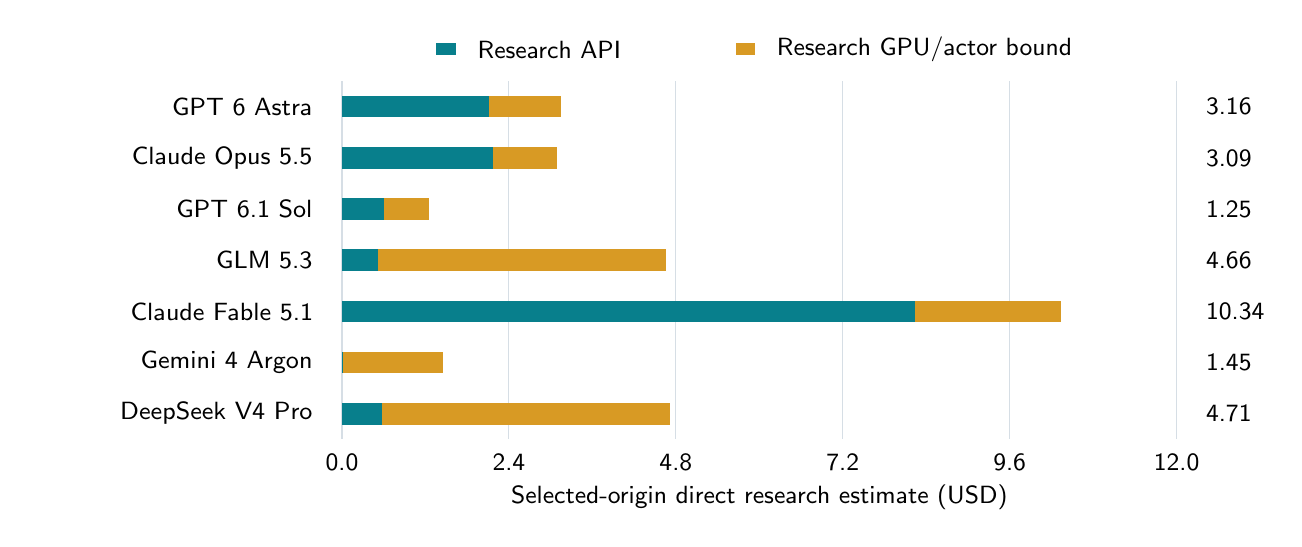
\begin{tikzpicture}[x=1cm,y=.65cm,font=\sffamily\small]
\draw[grid] (0.0000,.5)--(0.0000,-6.5);
\node[below] at (0.0000,-6.6) {0.0};
\draw[grid] (2.1200,.5)--(2.1200,-6.5);
\node[below] at (2.1200,-6.6) {2.4};
\draw[grid] (4.2400,.5)--(4.2400,-6.5);
\node[below] at (4.2400,-6.6) {4.8};
\draw[grid] (6.3600,.5)--(6.3600,-6.5);
\node[below] at (6.3600,-6.6) {7.2};
\draw[grid] (8.4800,.5)--(8.4800,-6.5);
\node[below] at (8.4800,-6.6) {9.6};
\draw[grid] (10.6000,.5)--(10.6000,-6.5);
\node[below] at (10.6000,-6.6) {12.0};
\node[anchor=east,text width=3.5cm,align=right] at (-.25, 0) {GPT 6 Astra};
\fill[teal] (0,-0.21) rectangle (1.86159, 0.21);
\fill[gold] (1.86159,-0.21) rectangle (2.78750, 0.21);
\node[anchor=west] at (10.85, 0) {3.16};
\node[anchor=east,text width=3.5cm,align=right] at (-.25,-1) {Claude Opus 5.5};
\fill[teal] (0,-1.21) rectangle (1.91295,-0.79);
\fill[gold] (1.91295,-1.21) rectangle (2.73269,-0.79);
\node[anchor=west] at (10.85,-1) {3.09};
\node[anchor=east,text width=3.5cm,align=right] at (-.25,-2) {GPT 6.1 Sol};
\fill[teal] (0,-2.21) rectangle (0.53248,-1.79);
\fill[gold] (0.53248,-2.21) rectangle (1.10082,-1.79);
\node[anchor=west] at (10.85,-2) {1.25};
\node[anchor=east,text width=3.5cm,align=right] at (-.25,-3) {GLM 5.3};
\fill[teal] (0,-3.21) rectangle (0.46143,-2.79);
\fill[gold] (0.46143,-3.21) rectangle (4.11905,-2.79);
\node[anchor=west] at (10.85,-3) {4.66};
\node[anchor=east,text width=3.5cm,align=right] at (-.25,-4) {Claude Fable 5.1};
\fill[teal] (0,-4.21) rectangle (7.28228,-3.79);
\fill[gold] (7.28228,-4.21) rectangle (9.13233,-3.79);
\node[anchor=west] at (10.85,-4) {10.34};
\node[anchor=east,text width=3.5cm,align=right] at (-.25,-5) {Gemini 4 Argon};
\fill[teal] (0,-5.21) rectangle (0.00746,-4.79);
\fill[gold] (0.00746,-5.21) rectangle (1.27803,-4.79);
\node[anchor=west] at (10.85,-5) {1.45};
\node[anchor=east,text width=3.5cm,align=right] at (-.25,-6) {DeepSeek V4 Pro};
\fill[teal] (0,-6.21) rectangle (0.50481,-5.79);
\fill[gold] (0.50481,-6.21) rectangle (4.16287,-5.79);
\node[anchor=west] at (10.85,-6) {4.71};
\fill[teal] (1.2, 1.0) rectangle (1.45, 1.25);\node[anchor=west] at (1.6, 1.12) {Research API};
\fill[gold] (5.0, 1.0) rectangle (5.25, 1.25);\node[anchor=west] at (5.4, 1.12) {Research GPU/actor bound};
\node[below] at (5.3,-7.2) {Selected-origin direct research estimate (USD)};
\end{tikzpicture}\caption{Known native research API estimates plus requested-resource research-clock bounds. API waits consume the resident GPU/actor clock even when a provider fails. Readiness, original finals, all common-A verification, shared idle/setup, CPU broker, storage and unresolved reserves remain separate. This is attribution within observed resources, not an additional bill added to lifecycle totals.}\end{figure}

\small\begin{tabularx}{\linewidth}{@{}Xrrrrr@{}}\toprule\textbf{Model} & \textbf{\shortstack[r]{Research\\API}} & \textbf{\shortstack[r]{Research\\compute}} & \textbf{\shortstack[r]{Direct\\research}} & \textbf{\shortstack[r]{Old R1\\final}} & \textbf{\shortstack[r]{Shared A\\validation}}\\\midrule

GPT 6 Astra & 2.11 & 1.05 & 3.16 & 0.37 & 0.37\\

Claude Opus 5.5 & 2.17 & 0.93 & 3.09 & 0.37 & 0.37\\

GPT 6.1 Sol & 0.60 & 0.64 & 1.25 & 0.36 & 0.35\\

GLM 5.3 & 0.52 & 4.14 & 4.66 & 0.39 & 0.37\\

Claude Fable 5.1 & 8.24 & 2.09 & 10.34 & 0.38 & 0.39\\

Gemini 4 Argon & 0.01 & 1.44 & 1.45 & 0.39 & 0.39\\

DeepSeek V4 Pro & 0.57 & 4.14 & 4.71 & 0.00 & 0.37\\

\bottomrule\end{tabularx}\normalsize

Primary model cost uses only its selected authoring origin: original R1 research for the retained six, and new R2 research for Deep. The prior Deep pilot is excluded from that ranking. Original final evaluations and all A common-board evaluations remain separate validation attribution. These phase estimates are never added again to lifecycle rental totals.

The new ledger carries the whole R1 known API balance of \$36.451673180 and unresolved reserve of \$362.00 once. This carryover includes retained source-attempt costs, older engineering and the aborted Deep pilot; it is not all newly generated work or all unallocated engineering. Current global known API estimate is \$37.023377544, with unresolved reserves \$392.00 separate from bills.

Compute quantities use captured Modal tariffs and requested 8 physical-core / 32 GiB boxes. Shared setup, baseline, idle, old/new sandbox lifetimes, CPU broker, storage and unobserved fees require independent actual resource accounting. Unknowns are not set to zero. Codex/orchestration/report-authoring charges are not observed by this ledger.

\subsection{Whole-task observed resource reconciliation}

This total includes earlier engineering as well as the seven selected authoring outcomes. Native API openings, phase attributions and earlier subtotals are counted once. Component labels are broad cost categories; no account, project, machine, storage or billing identifiers are published.

\small\begin{tabularx}{\linewidth}{@{}Xr@{}}\toprule\textbf{Captured known component} & \textbf{USD estimate}\\\midrule

Earlier accelerator engineering & 238.753596\\

Earlier CPU and storage auxiliaries & 0.025571\\

Cache storage & 0.017524\\

Pre-study runtime setup & 1.312442\\

Initial research runtime & 13.596043\\

Whole native API ledger, openings once & 37.023378\\

Common verification and recovery runtime & 8.588549\\

Trusted controller runtime and storage & 0.940597\\

\midrule Captured known subtotal & 300.257699\\

\bottomrule\end{tabularx}\normalsize

The captured known subtotal is \$300.26. The \$392 unresolved native reserve is separate; it is not added as a bill. Older unresolved holds contribute \$302 and selected GLM/Gemini/Deep requests contribute \$30 each.

These are source-bound public-tariff/requested-resource observation estimates, not invoices. Modal terminal poll timestamps verify absence of live resources and do not replace recorded lifecycle endpoints. The broker CPU estimate applies the documented 60-second minimum and one-second increments; boot deletion operation end supplies a qualified storage-window upper endpoint.

Still unpriced: exact tiny-probe allocation/CPU/RAM, two CPU timeout-probe exact lifetimes, Modal image build/import/network/storage adjustments, possible cache restore/network fees, taxes and account credits/discounts. The CPU-probe native-cap scenario of \$0.047592 and two-full 256 GiB restore sensitivity of \$25.60 are excluded from known costs. Shared actor research durations are attribution bounds; they are not independently added bills.

\subsection{Private audit and public replay boundary}

The private audit records closure of all task-owned rented execution resources and erasure of temporary credential copies. This edition excludes cloud ownership, IAM, account, operation and cleanup records. Independent public replay checks saved numerical observations and transformed-file integrity; it does not repeat the private infrastructure or source-provenance adjudication.

\section{Kernel workload and mathematical score}

\begin{figure}[H]\centering
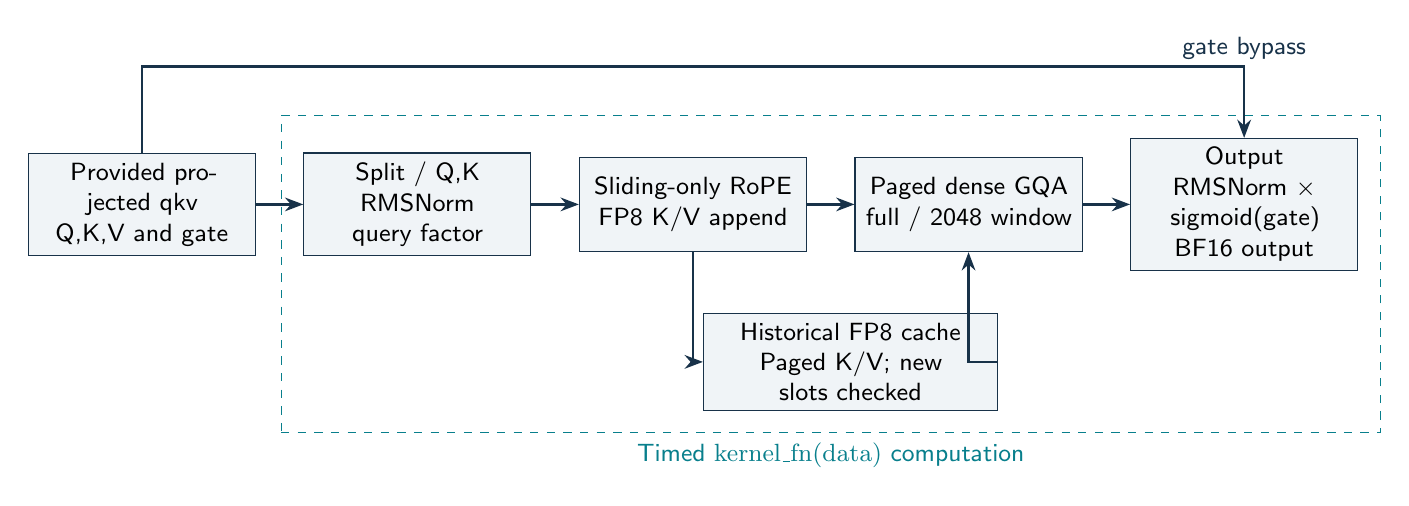
\begin{tikzpicture}[x=1cm,y=1cm,font=\sffamily\small,stage/.style={draw=navy,fill=pale,text width=2.65cm,minimum height=1.2cm,align=center},arrow/.style={-{Stealth},thick,navy}]
\node[stage] (in) at (0, 0) {Provided projected qkv\\Q,K,V and gate};
\node[stage] (norm) at (3.5, 0) {Split / Q,K RMSNorm\\query factor};
\node[stage] (rope) at (7, 0) {Sliding-only RoPE\\FP8 K/V append};
\node[stage] (attn) at (10.5, 0) {Paged dense GQA\\full / 2048 window};
\node[stage] (out) at (14, 0) {Output\\RMSNorm $\times$ sigmoid(gate)\\BF16 output};
\draw[arrow] (in)--(norm);\draw[arrow] (norm)--(rope);\draw[arrow] (rope)--(attn);\draw[arrow] (attn)--(out);
\draw[arrow] (in.north)--++(0, 1.1)-|node[above,pos=.52]{gate bypass}(out.north);
\node[stage,text width=3.5cm] (cache) at (9,-2) {\mbox{Historical FP8 cache}\\Paged K/V; new slots checked};
\draw[arrow] (rope.south)|-(cache.west);\draw[arrow] (cache.east)-|(attn.south);
\begin{scope}[on background layer]\node[draw=teal,dashed,fit=(norm)(rope)(attn)(out)(cache),inner sep=8pt,label={[text=teal]below:Timed $\mathrm{kernel\_fn(data)}$ computation}] {};\end{scope}
\end{tikzpicture}
\caption{Mathematical dataflow, not a launch-count diagram. QKV projection outputs are already supplied: no QKV weight GEMM is timed. Only Q/K are normalized; V and gate bypass that normalization. Sliding layers apply RoPE, full layers do not. All required keys/values and causal verify tokens remain in attention. Models can fuse stages or reuse FA3; precision boundaries are reviewed separately.}
\end{figure}

The 12 timed shapes form six decode/verify loads at B1/B16/B32. Each load weights sliding/full attention 46/16 before taking the geometric mean of six load ratios. It is not the unweighted average of 12 case speedups and does not measure end-to-end serving throughput.

\[B_l=46b_{l,\rm sliding}+16b_{l,\rm full},\quad C_l=46c_{l,\rm sliding}+16c_{l,\rm full},\quad S=\exp\left(\frac16\sum_l\log(B_l/C_l)\right).\]

Every passing score is reconstructed from saved calibration events, AB/BA replay pairs, shape statistics, weighted loads and seeded bootstrap samples with the hash-verified pure scoring helper. This CPU consistency check is not a new GPU measurement. Hosted seeds/calibration/anti-cheat remain unavailable; no exact hosted-judge equivalence is asserted.

\section{Experimental protocol and measurement limits}

Native model inference ran on provider APIs. H200s ran the generated attention kernels, not the language-model weights. A trusted CPU-only broker held scoped RAM credentials, native conversation state, clocks and budgets; workload sandboxes had no provider keys. No credentials or native conversations are included in this release.

\small\begin{tabularx}{\linewidth}{@{}lX@{}}\toprule\textbf{Dimension} & \textbf{Recorded contract}\\\midrule

Authoring & One selected source-attempt per model, maximum 1800 seconds; six retained R1 outcomes plus new Deep recovery. Prior interrupted Deep pilot remains separate.\\

Native context & Last 8 rounds, 120000 serialized UTF-8 bytes, 128000 native input tokens observed after response; native state resets on pruning. This heuristic does not equalize semantic context.\\

Native reasoning & High effort and 32768 output tokens per request. Equal effort names do not establish equal hidden compute.\\

Tools & JSON shell, GPU diagnostic, done. At most 3 diagnostics and 1--2 public scored cases per diagnostic; frozen derived seeds/reduced timing. No web/native provider tools.\\

CPU actors & Fresh Modal gVisor sandbox, 8 physical cores and 32 GiB requested/limited, UID/GID 65534, empty extra groups, no\_new\_privs, RLIMIT\_NPROC 256.\\

Isolation & Public/metadata network blocked; no GPU in actor, oracle/evaluator mount, identity token, credentials, other trials or Docker socket. Root-owned base plus private workspace/scratch.\\

GPU execution & H200 SXM; new process/private scratch/compiler caches per invocation; quiescence/cleanup between jobs. Common-A first full measurements only; B is Deep diagnostics/control only.\\

Final evaluation & Outside learning clock; 900-second worker limit plus trusted administrative/recovery margin. Real queue/worker durations are separately recorded.\\

Runtime & Torch 2.14.1+cu130, CUDA 13.0, driver 610.57.04, fixed SGLang source fingerprint; unique image, sandbox and hardware identifiers withheld.\\

\bottomrule\end{tabularx}\normalsize

Modal physical cores differ from Docker CPU-time quotas. gVisor, root-owned filesystem permissions and process limits are explicit substitutions for historical Docker isolation. Runtime identities were checked in the private audit. The immutable registry base was a launcher-request declaration, not Docker inspection of the old image. This public projection retains software versions and numerical/evaluator fingerprints while omitting unique infrastructure identities.

Sixteen mandatory cases test dtype/shape, mutation boundaries, edge values and graph replay after changed contents. Twelve scored cases additionally check candidate and baseline outputs after every fresh replay. New FP8 K/V entries have a separate 8 percent error bound; output uses the adaptive relative-L2 threshold $\min(0.15,\max(0.03, 2.5e_{\rm FP8\ query}+0.015))$, with row/near-zero and NaN/Inf safeguards.

Scored timing uses 20 alternating AB/BA CUDA-graph repetitions, a 128 MiB read reduction before every individual replay and 10 adjacent swapped pairs. Shape speedup is the median paired ratio; corrected baseline shape time is its median and candidate shape time is baseline/speedup. Nonpositive corrected times are rejected, not clamped.

The common-A empty-graph median was 3.232 microseconds. The public description gives about 4 microseconds, but the hosted calibration algorithm is unavailable. Local 95 percent intervals use 2000 independent per-shape swapped-pair bootstrap resamples and a 1.5 percent relative floor; overhead-calibration uncertainty is not included.

The report reconstructs calibration medians, all raw AB/BA summaries, weighted loads and seeded bootstrap intervals with the hash-verified Torch-free scoring helper. The public records are an explicit field-whitelisted projection of the first returned results. Their new hashes identify the projected data, not byte-exact administrative captures. These checks establish saved-data consistency, not a new GPU execution, public source adjudication or hosted-judge attestation.

The public task/seed and one selected artifact per model do not support a general model-ability ranking. Provider deadlines, hidden reasoning compute, tokenization/context and source-authoring board/tail policy remain material differences. No serving throughput or challenge-winning score is inferred.

\section{Source mechanisms and measured load drivers}

\begin{figure}[H]\centering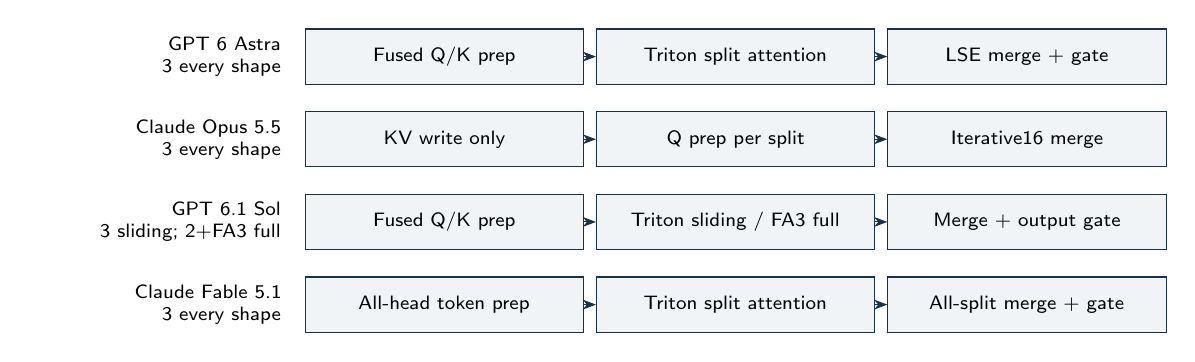
\begin{tikzpicture}[font=\sffamily\scriptsize,stage/.style={draw=navy,fill=pale,text width=3.3cm,minimum height=.7cm,align=center},link/.style={-{Stealth},navy}]
\node[anchor=east,text width=3.1cm,align=right] at (-.3, 0.0) {GPT 6 Astra\\3 every shape};
\node[stage] (s00) at (1.65, 0.0) {Fused Q/K prep};
\node[stage] (s01) at (5.35, 0.0) {Triton split attention};
\draw[link] (s00)--(s01);
\node[stage] (s02) at (9.05, 0.0) {LSE merge + gate};
\draw[link] (s01)--(s02);
\node[anchor=east,text width=3.1cm,align=right] at (-.3,-1.05) {Claude Opus 5.5\\3 every shape};
\node[stage] (s10) at (1.65,-1.05) {KV write only};
\node[stage] (s11) at (5.35,-1.05) {Q prep per split};
\draw[link] (s10)--(s11);
\node[stage] (s12) at (9.05,-1.05) {Iterative16 merge};
\draw[link] (s11)--(s12);
\node[anchor=east,text width=3.1cm,align=right] at (-.3,-2.1) {GPT 6.1 Sol\\3 sliding; 2+FA3 full};
\node[stage] (s20) at (1.65,-2.1) {Fused Q/K prep};
\node[stage] (s21) at (5.35,-2.1) {Triton sliding / FA3 full};
\draw[link] (s20)--(s21);
\node[stage] (s22) at (9.05,-2.1) {Merge + output gate};
\draw[link] (s21)--(s22);
\node[anchor=east,text width=3.1cm,align=right] at (-.3,-3.1500000000000004) {Claude Fable 5.1\\3 every shape};
\node[stage] (s30) at (1.65,-3.1500000000000004) {All-head token prep};
\node[stage] (s31) at (5.35,-3.1500000000000004) {Triton split attention};
\draw[link] (s30)--(s31);
\node[stage] (s32) at (9.05,-3.1500000000000004) {All-split merge + gate};
\draw[link] (s31)--(s32);
\end{tikzpicture}\caption{Source-visible custom launch structure of the four authored implementations. The Sol full-attention path uses FA3; its internal library launch count is not enumerated. These are static mechanisms, not hardware profiling or causal fusion ablations. Exact source hashes and source-audit precision qualifications are retained.}\end{figure}

The static observations below were checked against the four exact authored source hashes in the private audit. Source bodies are omitted from this public edition because their redistribution terms are not established; the observations cannot be independently re-adjudicated from this release alone. Timing attribution uses only their new common-A results. No occupancy, bandwidth, register-pressure profile or causal fusion ablation was run. FA3 internal launches are not counted as visible custom launches.

\subsection*{GPT 6 Astra}

Fully custom Triton dense paged grouped-query attention. Every scored path uses the same three-stage pipeline; no FA3 or other attention library invocation.

Memory/scheduling: Explicit BF16 Q plus FP32 Partial [B*L,Hq,S,D] and LSE [B*L,Hq,S]; scratch allocates actual query rows even though compute tile M=max(16,nextpow2(L*G)) pads decode to 16. Merge reads every split for each real query-head row. No input-derived cross-call cache.

Precision/source qualification: Lines 56-65 retain normalized Q/K activations in FP32 through interleaved RoPE, then BF16-round at line 67. The SGLang baseline BF16-rounds normalized activations before RoPE. This differs from the older frozen TASK wording requiring BF16 at the baseline BF16 activation points. The current KERNEL rules permit BF16 or FP32 there, so this is eligible under current rules but not strict frozen-TASK precision conformance. Legitimate FP32 RMS/softmax statistics and reductions are not themselves the caveat.

\subsection*{Claude Opus 5.5}

Fully custom three-kernel Triton attention on all shapes. Separate KV-only insertion; query preparation fused into each active split; split merge fused with RMSNorm/gate. No FA3 or other attention library invocation.

Memory/scheduling: Uses FP32 numerator, maximum and denominator scratch padded to query-tile rows. Decode pads eight real rows to 16 and writes the padding; verify uses 64 rows. Query preparation is repeated per active split, avoiding a query buffer. Merge writes gated output directly. Only configuration/device constants are cached across calls.

Precision/source qualification: The new source keeps normalized K in FP32 through RoPE and casts directly to FP8 cache at lines 106-124; query normalization/scale/RoPE stays FP32 until the BF16 query cast at line 173. It also sends the FP32 merged attention value directly into output RMSNorm at lines 251-252, omitting the baseline BF16 attention-output rounding. These activation choices are permitted by current KERNEL BF16-or-FP32 allowances, but differ from the older frozen TASK requirement to keep BF16 at baseline BF16 activation points. FP32 RMS/softmax reduction statistics themselves are legitimate and are not the caveat.

\subsection*{GPT 6.1 Sol}

Hybrid attention: fused Q/K preparation/cache insertion; custom dense split attention only for sliding layers; installed FA3 on every full-context shape, including B1 decode. This is independently read from the fresh source, not the old R3 Sol dispatch.

Memory/scheduling: BF16/FP8 query staging plus sliding FP32 normalized partials and LSE [B,Hkv,NS,M,D] / [B,Hkv,NS,M]. Decode M16 stores padding beyond eight real rows; verify M64 is fully used. No sliding scratch is allocated on full paths. No input-derived cross-call cache.

Precision/source qualification: In \_prepare, normalized Q/K and the partner component remain FP32 through interleaved RoPE; BF16 activation rounding occurs only after rotation. The baseline BF16-rounds normalized activations before RoPE. Current KERNEL rules permit BF16 or FP32 at those points, but the older frozen TASK requires BF16 where the baseline keeps it. This fresh Sol artifact therefore differs from strict frozen-TASK precision even though its post-RoPE, pre-cache and pre-output-RMS BF16 rounding is retained. Legitimate FP32 RMS/softmax reductions are not the caveat.

\subsection*{Claude Fable 5.1}

Fully custom three-kernel Triton dense paged GQA attention for both full and sliding layers. Separate fused per-token Q/K preparation/cache insertion and BF16 Q staging; split attention; vectorized merge/norm/gate. No FA3 or other attention-library call. This is read from the fresh source and differs from the old two-kernel R3 Fable artifact.

Memory/scheduling: Q staging plus FP32 numerator [B,Hkv,NSPLIT,M\_PAD,D] and max/denominator arrays. Decode M\_PAD 16 reserves two times the eight real query rows, but stores mask padded rows. Verify M\_PAD 64 holds all real rows. The merge loads every split for valid query rows in a single power-of-two-padded vector, with 8 warps when NSPLIT\_PAD*D\textgreater{}8192 else 4. No cross-call input-derived cache.

Precision/source qualification: The preparation kernel retains normalized/scaled Q and normalized K in FP32 through interleaved RoPE. Q is BF16-rounded only afterward, while K is cast directly from FP32 to FP8 cache. The combine kernel also keeps merged attention in FP32 into output RMSNorm rather than first rounding attention to the baseline BF16 activation. Current KERNEL rules permit BF16 or FP32 at these points, but the older frozen TASK requires BF16 wherever the baseline keeps it. This is a precision-conformance difference, not prohibited cheating; FP32 reduction statistics themselves are legitimate.

The three unchanged targets share the official PyTorch starter. It gathers/promotes the page-table-capacity K/V tensors, forms dense attention intermediates and loops over requests. Those source facts describe the supplied control, not strategies authored by GLM, Gemini or Deep. Their tiny raw ratios are retained only in the appendix.

\section{Source audits and limits}

Dated kernel-rule observation from 9 November 2026: BF16 or FP32 activations are allowed at baseline BF16 activation points. Serving restrictions are a separate contract. The older frozen TASK text and measured sources were not changed.

\subsection*{GPT 6 Astra}

Reviewed source SHA256: \hash{18e4e4865b0be77ff44a6c4a4ad06ff2c2ac75da5d5b64461b3b793f1d95700b}.


Lines 56-65 retain normalized Q/K activations in FP32 through interleaved RoPE, then BF16-round at line 67. The SGLang baseline BF16-rounds normalized activations before RoPE. This differs from the older frozen TASK wording requiring BF16 at the baseline BF16 activation points. The current KERNEL rules permit BF16 or FP32 there, so this is eligible under current rules but not strict frozen-TASK precision conformance. Legitimate FP32 RMS/softmax statistics and reductions are not themselves the caveat.

\subsection*{Claude Opus 5.5}

Reviewed source SHA256: \hash{4755401a2e7c09db8f5dc51a13c29ee69d832dbf0683036f9b31b6014334a473}.


The new source keeps normalized K in FP32 through RoPE and casts directly to FP8 cache at lines 106-124; query normalization/scale/RoPE stays FP32 until the BF16 query cast at line 173. It also sends the FP32 merged attention value directly into output RMSNorm at lines 251-252, omitting the baseline BF16 attention-output rounding. These activation choices are permitted by current KERNEL BF16-or-FP32 allowances, but differ from the older frozen TASK requirement to keep BF16 at baseline BF16 activation points. FP32 RMS/softmax reduction statistics themselves are legitimate and are not the caveat.

\subsection*{GPT 6.1 Sol}

Reviewed source SHA256: \hash{c420bad454751564638731bc928bd36c79a11afe22a5a61dabff6f6f639844cf}.


In \_prepare, normalized Q/K and the partner component remain FP32 through interleaved RoPE; BF16 activation rounding occurs only after rotation. The baseline BF16-rounds normalized activations before RoPE. Current KERNEL rules permit BF16 or FP32 at those points, but the older frozen TASK requires BF16 where the baseline keeps it. This fresh Sol artifact therefore differs from strict frozen-TASK precision even though its post-RoPE, pre-cache and pre-output-RMS BF16 rounding is retained. Legitimate FP32 RMS/softmax reductions are not the caveat.

\subsection*{GLM 5.3}

Reviewed source SHA256: \hash{1c3828573c362989db3385eff9a5b67a7c66d6503e9e242d28f9b150f6fb9472}.


Inherited starter rms() returns FP32 normalized Q/K, retained through RoPE; Q is BF16-rounded only afterward and normalized K is cast directly to FP8 cache without the baseline BF16 activation rounding. Current KERNEL rules permit these FP32 activations, but they differ from the older frozen TASK BF16-at-baseline-points wording. This caveat is inherited byte-for-byte from the provided starter, not a GLM-created precision optimization or evidence of cheating. Legitimate FP32 reduction statistics are not the caveat.

Primary eligibility exclusions: research did not complete under its declared policy; provider timeout/failure; no modified submission.

\subsection*{Claude Fable 5.1}

Reviewed source SHA256: \hash{2f77e16261da9d91970c29977580f25c2a26224bb4b90f451fba2cc52bbf2198}.


The preparation kernel retains normalized/scaled Q and normalized K in FP32 through interleaved RoPE. Q is BF16-rounded only afterward, while K is cast directly from FP32 to FP8 cache. The combine kernel also keeps merged attention in FP32 into output RMSNorm rather than first rounding attention to the baseline BF16 activation. Current KERNEL rules permit BF16 or FP32 at these points, but the older frozen TASK requires BF16 wherever the baseline keeps it. This is a precision-conformance difference, not prohibited cheating; FP32 reduction statistics themselves are legitimate.

\subsection*{Gemini 4 Argon}

Reviewed source SHA256: \hash{1c3828573c362989db3385eff9a5b67a7c66d6503e9e242d28f9b150f6fb9472}.


The inherited rms() returns FP32 normalized Q/K, retained through interleaved RoPE; Q is BF16-rounded only afterward, and normalized K is converted directly to FP8 cache without the baseline BF16 activation rounding. These FP32 choices are current-KERNEL eligible, but differ from the older frozen TASK BF16-at-baseline-points wording. The difference is inherited from the supplied starter, not a Gemini-created precision optimization or evidence of cheating. FP32 reductions themselves are legitimate.

Primary eligibility exclusions: research did not complete under its declared policy; provider timeout/failure; no modified submission.

\subsection*{DeepSeek V4 Pro}

Reviewed source SHA256: \hash{1c3828573c362989db3385eff9a5b67a7c66d6503e9e242d28f9b150f6fb9472}.


The inherited rms() returns FP32 normalized Q/K, retained through interleaved RoPE; Q is BF16-rounded only afterward, and normalized K is converted directly to FP8 cache without baseline BF16 activation rounding. Current KERNEL rules allow these FP32 choices. Strict older frozen TASK BF16-at-baseline-points conformance is false as an inherited starter property; it is not a DeepSeek-created precision optimization or evidence of cheating. Ordinary FP32 reductions are legitimate.

Primary eligibility exclusions: research did not complete under its declared policy; provider timeout/failure; no modified submission.

Current kernel BF16-or-FP32 permission and older frozen-TASK BF16 round-point conformance are separate. An inherited starter does not establish a precision modification authored by the provider. These are dated review observations from the private audit. The public edition links the upstream rules and does not certify current organizer approval or serving-track eligibility.

The retained six and recovered Deep do not share an identical uninterrupted authoring run: board allocation, wall-clock time and administrative tail policy differ. Deep had an earlier interrupted pilot whose context/code/feedback are not reused. One task and one selected source per model cannot establish general kernel-authoring ability or a statistically robust model ranking.

\appendix\section{Recorded protocol and source lineage}

\subsection{Inherited-starter observations, not model points}

\small\begin{tabularx}{\linewidth}{@{}Xrrr@{}}\toprule\textbf{Inherited control} & \textbf{Raw A ratio} & \textbf{95\% low} & \textbf{95\% high}\\\midrule

GLM 5.3 & 0.00247669 & 0.00243953 & 0.00251384\\

Gemini 4 Argon & 0.00246886 & 0.00243183 & 0.00250589\\

DeepSeek V4 Pro & 0.00247153 & 0.00243445 & 0.00250860\\

\bottomrule\end{tabularx}\normalsize

These all passed 28 oracle cases, but no modified final kernel was delivered. They are observations of the same inherited bytes, not slow kernels authored by those providers and not zero-valued failures.

\subsection{Secondary original-R1 timings}

The following original measurements are fixed secondary evidence. Common-A values above are always primary, regardless of which is faster.

\small\begin{tabularx}{\linewidth}{@{}Xr@{\hspace{12pt}}r@{}}\toprule\textbf{Retained source} & \textbf{Original R1} & \textbf{Common A}\\\midrule

GPT 6 Astra & 1.176561 & 1.177731\\

Claude Opus 5.5 & 0.974758 & 0.973412\\

GPT 6.1 Sol & 1.270508 & 1.270167\\

GLM 5.3 & 0.002452 & 0.002477\\

Claude Fable 5.1 & 1.159929 & 1.156184\\

Gemini 4 Argon & 0.002456 & 0.002469\\

\bottomrule\end{tabularx}\normalsize

\subsection{Public runtime facts and replay scope}

\small\begin{tabularx}{\linewidth}{@{}lX@{}}\toprule\textbf{Scientific field} & \textbf{Recorded value}\\\midrule
Hardware & NVIDIA H200 SXM; one visible GPU; Hopper compute capability 9.0\\
Execution & Native gVisor sandbox; GPU role A for all first final reports\\
Torch / CUDA / driver & 2.14.1+cu130 / 13.0 / 610.57.04\\
Pure scoring SHA256 & \hash{3e3f748300e8ba187bb755c1a7c9fc7bc1d5221b8cec9cfde55a855ab14c8a29}\\
Evaluator SHA256 & \hash{01cd6fa219a93546a9a59fdc66c5b2fe9f64499a1188f9f44fb4ca62b99e7af5}\\
Protocol SHA256 & \hash{2657569846a13b1c91f5d4c0345144c79464a793116f5047a44b107b734b5116}\\
SGLang source SHA256 & \hash{3f70ce2858c43b2d830379de0b9a32f5f4e4e950191ef3c2bc9d6e0c264d4ce7}\\
\bottomrule\end{tabularx}\normalsize

\subsection{A derived public release}

The public dataset uses generic model and board-role labels. It retains every calibration scalar, AB/BA replay pair, mandatory-case outcome, scored-case observation, weighted-load summary and score interval needed by the independent CPU numerical replay. Public hashes are recomputed for these derived records. Original captures and their unchanged provenance graph remain private.

The public projection removes work-email addresses, local usernames and paths, machine names, IP addresses, cloud projects and accounts, service identities, unique hardware and object IDs, request/operation identifiers, commands, stderr and administrative records. Native conversation state, provider keys, credential files, raw IAM records and actor working trees are not distributed.

Numerical reconstruction does not prove that a GPU event occurred. The private source review and infrastructure checks are author-reported facts here, rather than independently replayable public attestations. No original candidate source, diagnostic candidate, problem statement, starter, reference or baseline body is included. Upstream hash/URL references and an optional explicit local acquisition path are supplied separately under their original terms; the harness MIT license does not relicense them.

To reproduce the saved-data checks, run the included CPU replay script. To rebuild this paper, install Tectonic and the documented PDF dependency, then run the public report builder. Neither operation calls a model, provisions a resource, imports a candidate, requires API keys or reads the private workspace. The source archive contains only files from the public release and its own payload manifest.

Core references: \href{https://openkernelchallenge.dev/problems/muse_attention_decode}{official problem}; \href{https://openkernelchallenge.dev/rules\#kernels}{kernel rules}; \href{https://modal.com/pricing}{Modal pricing}; \href{https://modal.com/docs/guide/gpu}{GPU hardware}; \href{https://modal.com/docs/guide/resources}{sandbox resources}. These links provide context, not a new redistribution grant. Recorded costs and rule observations remain dated study facts, not assertions of current pricing or a hosted score.

\clearpage\subsection{Public numerical case definitions}

\footnotesize\begin{longtable}{@{}p{.13\linewidth}p{.30\linewidth}p{.51\linewidth}@{}}\toprule\textbf{Case} & \textbf{Load/weight} & \textbf{Shape arguments}\\\midrule\endhead

test-01 & mandatory & batch=1, ctx=10, heads=tp8, layer=sliding\\

test-02 & mandatory & batch=3, ctx=2047, heads=tp8, layer=sliding\\

test-03 & mandatory & batch=5, ctx=5000, heads=tp8, layer=sliding, q\_len=8, spread=mixed, page=1\\

test-04 & mandatory & batch=4, ctx=3000, heads=tp8, layer=full\\

test-05 & mandatory & batch=8, ctx=8192, heads=dp, layer=full, spread=mixed\\

test-06 & mandatory & batch=2, ctx=100000, heads=tp8, layer=full, q\_len=8, page=1\\

test-07 & mandatory & batch=4, ctx=6000, heads=tp8, layer=sliding, dist=edges, page=1\\

test-08 & mandatory & batch=4, ctx=6000, heads=tp8, layer=full, q\_len=8, dist=edges\\

test-09 & mandatory & batch=1, ctx=1048576, heads=tp8, layer=full, q\_len=8\\

test-10 & mandatory & batch=3, ctx=4000, heads=tp8, layer=sliding, q\_len=8, page=1, kv\_scale=0.015625\\

test-11 & mandatory & batch=2, ctx=9000, heads=tp8, layer=full, kv\_scale=0.015625\\

test-12 & mandatory & batch=4, ctx=80000, heads=tp8, layer=full, spread=mixed, dist=soft\\

test-13 & mandatory & batch=4, ctx=6000, heads=tp8, layer=sliding, q\_len=8, dist=soft, page=1\\

test-14 & mandatory & batch=2, ctx=20000, heads=dp, layer=full, q\_len=8, dist=soft\\

test-15 & mandatory & batch=4, ctx=80000, heads=tp8, layer=full, spread=mixed, dist=coherent, page=1\\

test-16 & mandatory & batch=2, ctx=20000, heads=dp, layer=full, q\_len=8, dist=coherent\\

scored-01 & decode 1 / 46 & batch=1, ctx=80000, heads=tp8, layer=sliding, page=1, dist=soft\\

scored-02 & decode 1 / 16 & batch=1, ctx=80000, heads=tp8, layer=full, page=1, dist=coherent\\

scored-03 & decode 16 / 46 & batch=16, ctx=80000, heads=tp8, layer=sliding, page=1, spread=agentic, dist=soft\\

scored-04 & decode 16 / 16 & batch=16, ctx=80000, heads=tp8, layer=full, page=1, spread=agentic, dist=coherent\\

scored-05 & decode 32 / 46 & batch=32, ctx=80000, heads=tp8, layer=sliding, page=1, spread=agentic, dist=soft\\

scored-06 & decode 32 / 16 & batch=32, ctx=80000, heads=tp8, layer=full, page=1, spread=agentic, dist=coherent\\

scored-07 & verify 1 / 46 & batch=1, ctx=80000, heads=tp8, layer=sliding, page=1, q\_len=8, dist=soft\\

scored-08 & verify 1 / 16 & batch=1, ctx=80000, heads=tp8, layer=full, page=1, q\_len=8, dist=coherent\\

scored-09 & verify 16 / 46 & batch=16, ctx=80000, heads=tp8, layer=sliding, page=1, q\_len=8, spread=agentic, dist=soft\\

scored-10 & verify 16 / 16 & batch=16, ctx=80000, heads=tp8, layer=full, page=1, q\_len=8, spread=agentic, dist=coherent\\

scored-11 & verify 32 / 46 & batch=32, ctx=80000, heads=tp8, layer=sliding, page=1, q\_len=8, spread=agentic, dist=soft\\

scored-12 & verify 32 / 16 & batch=32, ctx=80000, heads=tp8, layer=full, page=1, q\_len=8, spread=agentic, dist=coherent\\

\bottomrule\end{longtable}\normalsize

\end{document}
